\documentclass[8pt]{beamer}
\usepackage[utf8]{inputenc}
\usepackage{ulem}
\usepackage{xcolor}
\usepackage{colortbl}
\usepackage{epsfig}
% \usepackage{cancel}
\usepackage{ulem}
% \usepackage{threeparttable} % Joao Pela: 
\usepackage{amsmath}
\usepackage{hyperref}
\usepackage{appendixnumberbeamer}
\usepackage{pdfpages}
% \usepackage{feynmp}         % For latex produced Feynman Diagrams

% Rule for feynmp diagrams to be considered graphics
% \DeclareGraphicsRule{*}{mps}{*}{}
% 
% % New compile sequence for feynmp
% \makeatletter
% \def\endfmffile{%
%   \fmfcmd{\p@rcent\space the end.^^J%
%           end.^^J%
%           endinput;}%
%   \if@fmfio
%     \immediate\closeout\@outfmf
%   \fi
%   \ifnum\pdfshellescape=\@ne
%     \immediate\write18{mpost \thefmffile}%
%   \fi}
% \makeatother

\usetheme{Madrid}

% Add support for \subsubsectionpage
\def\subsubsectionname{\translate{Subsubsection}}
\def\insertsubsubsectionnumber{\arabic{subsubsection}}
\setbeamertemplate{subsubsection page}
{
  \begin{centering}
    {\usebeamerfont{subsubsection name}\usebeamercolor[fg]{subsubsection name}\subsubsectionname~\insertsubsubsectionnumber}
    \vskip1em\par
    \begin{beamercolorbox}[sep=4pt,center]{part title}
      \usebeamerfont{subsubsection title}\insertsubsubsection\par
    \end{beamercolorbox}
  \end{centering}
}
\def\subsubsectionpage{\usebeamertemplate*{subsubsection page}}

\AtBeginSection{\frame{\sectionpage}}
\AtBeginSubsection{\frame{\subsectionpage}}
\AtBeginSubsubsection{\frame{\subsubsectionpage}}

\author[J. Pela]{J. Pela}
\title{Update on Trigger Studies for 2015 (Legacy System)}
\institute[ICL]{Imperial College London}
\date{2014-07-29}

% The log drawn in the upper right corner.
\logo{\includegraphics[height=0.115\paperheight]{img/Logo_CMSICL.png}}

\begin{document}
\setlength{\unitlength}{1mm}

% ###################################################
\begin{frame}
  \titlepage
\end{frame}

% ###################################################
\begin{frame}{Today's presentation}

\begin{block}{Topics}
 
\begin{itemize}
  \item Trigger signal efficiency (including higher ETM seeds) 
  \item L1 and HLT Rates and seed study.
  \item ECAL TT, HCAL TT and RCT Region saturation.
  \item ECAL TT peak investigation.
\end{itemize}

\end{block}

\end{frame}

\section{Introduction}

% ###################################################
\begin{frame}{Neutrino Gun (reminder)}

\begin{block}{Base idea}
 
For studying of L1T Rates the normal procedure is using neutrino gun samples. :
\begin{itemize}
 \item Hard process is invisible (only a neutrino is fired through the experiment)
 \item Event consists only of PU (overlapped Minimum/Zero bias events)
 \item Recreated the vast majority of events at the fire the L1T
\end{itemize}

\end{block}

\begin{block}{Method}
 
\begin{itemize}
 \item Determine algorithm event selection efficiency, this will be the probability of a bunch firing.
 \item Each bunch firing will represent 11246 Hz, so we apply efficiency and obtain rate per bunch.
 \item We multiply per number of bunches on the machine to obtain algorithm pure rate (no overlapping with other algorithm)
\end{itemize}
 
\end{block}

\end{frame}

% ###################################################
\begin{frame}{HLT Seeds}

\begin{block}{Information}
 
\begin{itemize}
  \item For full documentation purposes I have included what are the seeds for each one of our triggers available on the samples
  \item While looking into the menu details I have notices the presence of 2 additional prompt-like triggers with PFMETnoMu75. I added them to the study.
  \item Notice that all prompt triggers are seeded only by L1\_ETM40 and all parked by some combination of L1\_ETM and L1\_HTT.
\end{itemize}
 
\end{block}

\begin{block}{Map of seeds}
\centering

\resizebox{0.8\linewidth}{!}{
\begin{tabular}{|l||l|l|}
\hline
HLT Path & ETM Seeds & HTT Seeds \\
\hline \hline
HLT\_DiPFJet40\_PFMETnoMu65\_MJJ800VBF\_AllJets\_v     &  & L1\_ETM40 \\
HLT\_DiPFJet40\_PFMETnoMu65\_MJJ600VBF\_LeadingJets\_v &  & L1\_ETM40 \\
\hline \hline
HLT\_DiPFJet40\_PFMETnoMu75\_MJJ800VBF\_AllJets\_v     &  & L1\_ETM40 \\
HLT\_DiPFJet40\_PFMETnoMu75\_MJJ600VBF\_LeadingJets\_v &  & L1\_ETM40 \\    
\hline \hline
HLT\_DiJet20\_MJJ650\_AllJets\_DEta3p5\_HT120\_VBF\_v   & L1\_HTT200, L1\_HTT175             & L1\_ETM40, L1\_ETM50 \\
HLT\_DiJet30\_MJJ700\_AllJets\_DEta3p5\_VBF\_v          & L1\_HTT200, L1\_HTT175             & L1\_ETM40, L1\_ETM50 \\
HLT\_DiJet35\_MJJ650\_AllJets\_DEta3p5\_VBF\_v          & L1\_HTT200, L1\_HTT175, L1\_HTT150 & L1\_ETM40 \\
HLT\_DiJet35\_MJJ700\_AllJets\_DEta3p5\_VBF\_v          & L1\_HTT200, L1\_HTT175             & L1\_ETM40 \\
HLT\_DiJet35\_MJJ750\_AllJets\_DEta3p5\_VBF\_v          & L1\_HTT200, L1\_HTT175             & L1\_ETM40 \\
\hline 
\end{tabular}
}

\end{block}

\end{frame}

\section{VBF Signal efficiency}

% ###################################################
\begin{frame}{VBF Invisible - Efficiency}

\begin{columns}

\column[t]{0.40\linewidth}
\begin{block}{L1T}
\centering

\resizebox{1.0\linewidth}{!}{

\begin{tabular}{|c||c|c|c|}
\hline
L1T & PU20bx25 & PU40bx50 & PU40bx25 \\
\hline \hline
L1\_ETM30 & 0.592926 & 0.618057 & 0.649159 \\
L1\_ETM36 & 0.522186 & 0.543433 & 0.572288 \\
L1\_ETM40 & 0.480770 & 0.498892 & 0.526785 \\
L1\_ETM50 & 0.389255 & 0.402511 & 0.426774 \\
L1\_ETM70 & 0.254493 & 0.262797 & 0.280257 \\
L1\_ETM100 & 0.136494 & 0.139298 & 0.150268 \\
L1\_HTT150 & 0.146744 & 0.270042 & 0.480381 \\
L1\_HTT175 & 0.102455 & 0.198686 & 0.390660 \\
L1\_HTT200 & 0.071823 & 0.145055 & 0.313576 \\
\hline
\end{tabular}


}
\end{block}

\column[t]{0.55\linewidth}
\begin{block}{Notes}
 
\begin{itemize}
  \item Notice that from L1\_ETM40 to L1\_ETM70 the signal efficiency drops by $\sim50\%$ on all scenarios
  \item Also notice the decrease of efficiency on parked triggers as PU goes up and separation goes down.
\end{itemize}
 
\end{block}

\end{columns}

\begin{block}{HLT}
\centering
 
\resizebox{0.8\linewidth}{!}{  
\begin{tabular}{|c||c|c|c|}
\hline
HLT & PU20bx25 & PU40bx50 & PU40bx25 \\
\hline \hline
HLT\_DiPFJet40\_PFMETnoMu65\_MJJ800VBF\_AllJets\_v & 0.084993 & 0.087952 & 0.091972 \\
HLT\_DiPFJet40\_PFMETnoMu75\_MJJ800VBF\_AllJets\_v & 0.082599 & 0.085310 & 0.089228 \\
HLT\_DiPFJet40\_PFMETnoMu65\_MJJ600VBF\_LeadingJets\_v & 0.107917 & 0.109334 & 0.116750 \\
HLT\_DiPFJet40\_PFMETnoMu75\_MJJ600VBF\_LeadingJets\_v & 0.104735 & 0.105818 & 0.112964 \\
HLT\_DiJet20\_MJJ650\_AllJets\_DEta3p5\_HT120\_VBF\_v & 0.149766 & 0.137726 & 0.105392 \\
HLT\_DiJet30\_MJJ700\_AllJets\_DEta3p5\_VBF\_v & 0.127966 & 0.125063 & 0.077578 \\
HLT\_DiJet35\_MJJ650\_AllJets\_DEta3p5\_VBF\_v & 0.124930 & 0.119819 & 0.079295 \\
HLT\_DiJet35\_MJJ700\_AllJets\_DEta3p5\_VBF\_v & 0.114779 & 0.110012 & 0.069185 \\
HLT\_DiJet35\_MJJ750\_AllJets\_DEta3p5\_VBF\_v & 0.106152 & 0.102060 & 0.062001 \\
\hline
\end{tabular}

}

\end{block}

\end{frame}

% ###################################################
\begin{frame}{HLT Prompt paths with higher threshold seeds}

We can easilly obtain the efficiencies of our current HLT paths with an AND with higher L1\_ETM seeds.

\begin{block}{VBF Signal Efficiencies}
\centering

\resizebox{0.8\linewidth}{!}{
\begin{tabular}{|l||c|c|c|}
\hline
L1 + HLT Path & PU20bx25 & PU40bx50 & PU40bx25 \\
\hline\hline
L1\_ETM40 + HLT\_DiPFJet40\_PFMETnoMu65\_MJJ800VBF\_AllJets\_v      & 0.0849935 & 0.0878568 & 0.0919718 \\
L1\_ETM50 + HLT\_DiPFJet40\_PFMETnoMu65\_MJJ800VBF\_AllJets\_v      & 0.0768525 & 0.0796637 & 0.0839013 \\
L1\_ETM70 + HLT\_DiPFJet40\_PFMETnoMu65\_MJJ800VBF\_AllJets\_v      & 0.0614486 & 0.0634076 & 0.0677252 \\
L1\_ETM100 + HLT\_DiPFJet40\_PFMETnoMu65\_MJJ800VBF\_AllJets\_v     & 0.0411943 & 0.0422621 & 0.0466194 \\
\hline
L1\_ETM40 + HLT\_DiPFJet40\_PFMETnoMu65\_MJJ600VBF\_LeadingJets\_v  & 0.107917  & 0.10923   & 0.11675   \\
L1\_ETM50 + HLT\_DiPFJet40\_PFMETnoMu65\_MJJ600VBF\_LeadingJets\_v  & 0.0972576 & 0.0986653 & 0.105798  \\
L1\_ETM70 + HLT\_DiPFJet40\_PFMETnoMu65\_MJJ600VBF\_LeadingJets\_v  & 0.0761378 & 0.077375  & 0.0840711 \\
L1\_ETM100 + HLT\_DiPFJet40\_PFMETnoMu65\_MJJ600VBF\_LeadingJets\_v & 0.0486722 & 0.049405  & 0.055253  \\
\hline\hline
L1\_ETM40 + HLT\_DiPFJet40\_PFMETnoMu75\_MJJ800VBF\_AllJets\_v      & 0.0825993 & 0.085225  & 0.0892285 \\
L1\_ETM50 + HLT\_DiPFJet40\_PFMETnoMu75\_MJJ800VBF\_AllJets\_v      & 0.0750099 & 0.0776955 & 0.0817088 \\
L1\_ETM70 + HLT\_DiPFJet40\_PFMETnoMu75\_MJJ800VBF\_AllJets\_v      & 0.0605066 & 0.0623966 & 0.0665099 \\
L1\_ETM100 + HLT\_DiPFJet40\_PFMETnoMu75\_MJJ800VBF\_AllJets\_v     & 0.0409795 & 0.0419788 & 0.0462468 \\
\hline
L1\_ETM40 + HLT\_DiPFJet40\_PFMETnoMu75\_MJJ600VBF\_LeadingJets\_v  & 0.104735  & 0.105728  & 0.112964  \\
L1\_ETM50 + HLT\_DiPFJet40\_PFMETnoMu75\_MJJ600VBF\_LeadingJets\_v  & 0.0948593 & 0.0960417 & 0.102829  \\
L1\_ETM70 + HLT\_DiPFJet40\_PFMETnoMu75\_MJJ600VBF\_LeadingJets\_v  & 0.0749996 & 0.0761181 & 0.0824479 \\
L1\_ETM100 + HLT\_DiPFJet40\_PFMETnoMu75\_MJJ600VBF\_LeadingJets\_v & 0.0484408 & 0.0490825 & 0.0547934 \\
\hline
\end{tabular}
}

\end{block}

\begin{itemize}
  \item Going from seed L1\_ETM40 to L1\_ETM70 seed makes us lose about $\sim25\%$ signal efficiency at HLT, which is an improvement from about $\sim50\%$ at L1T 
  \item With seed L1\_ETM70 and PFMETnoMu75 at HLT means a reduction of efficiency of $\sim30\%$
\end{itemize}

\end{frame}

\section{L1 and HLT rates and seed study}

% ###################################################
\begin{frame}{Neutrino Gun - L1 Quantities}

Here we can see the relevant seed L1 quantities evolution for each scenario:

\begin{columns}

\column[t]{0.45\linewidth}
\begin{block}{L1T ETM}
 
\centering
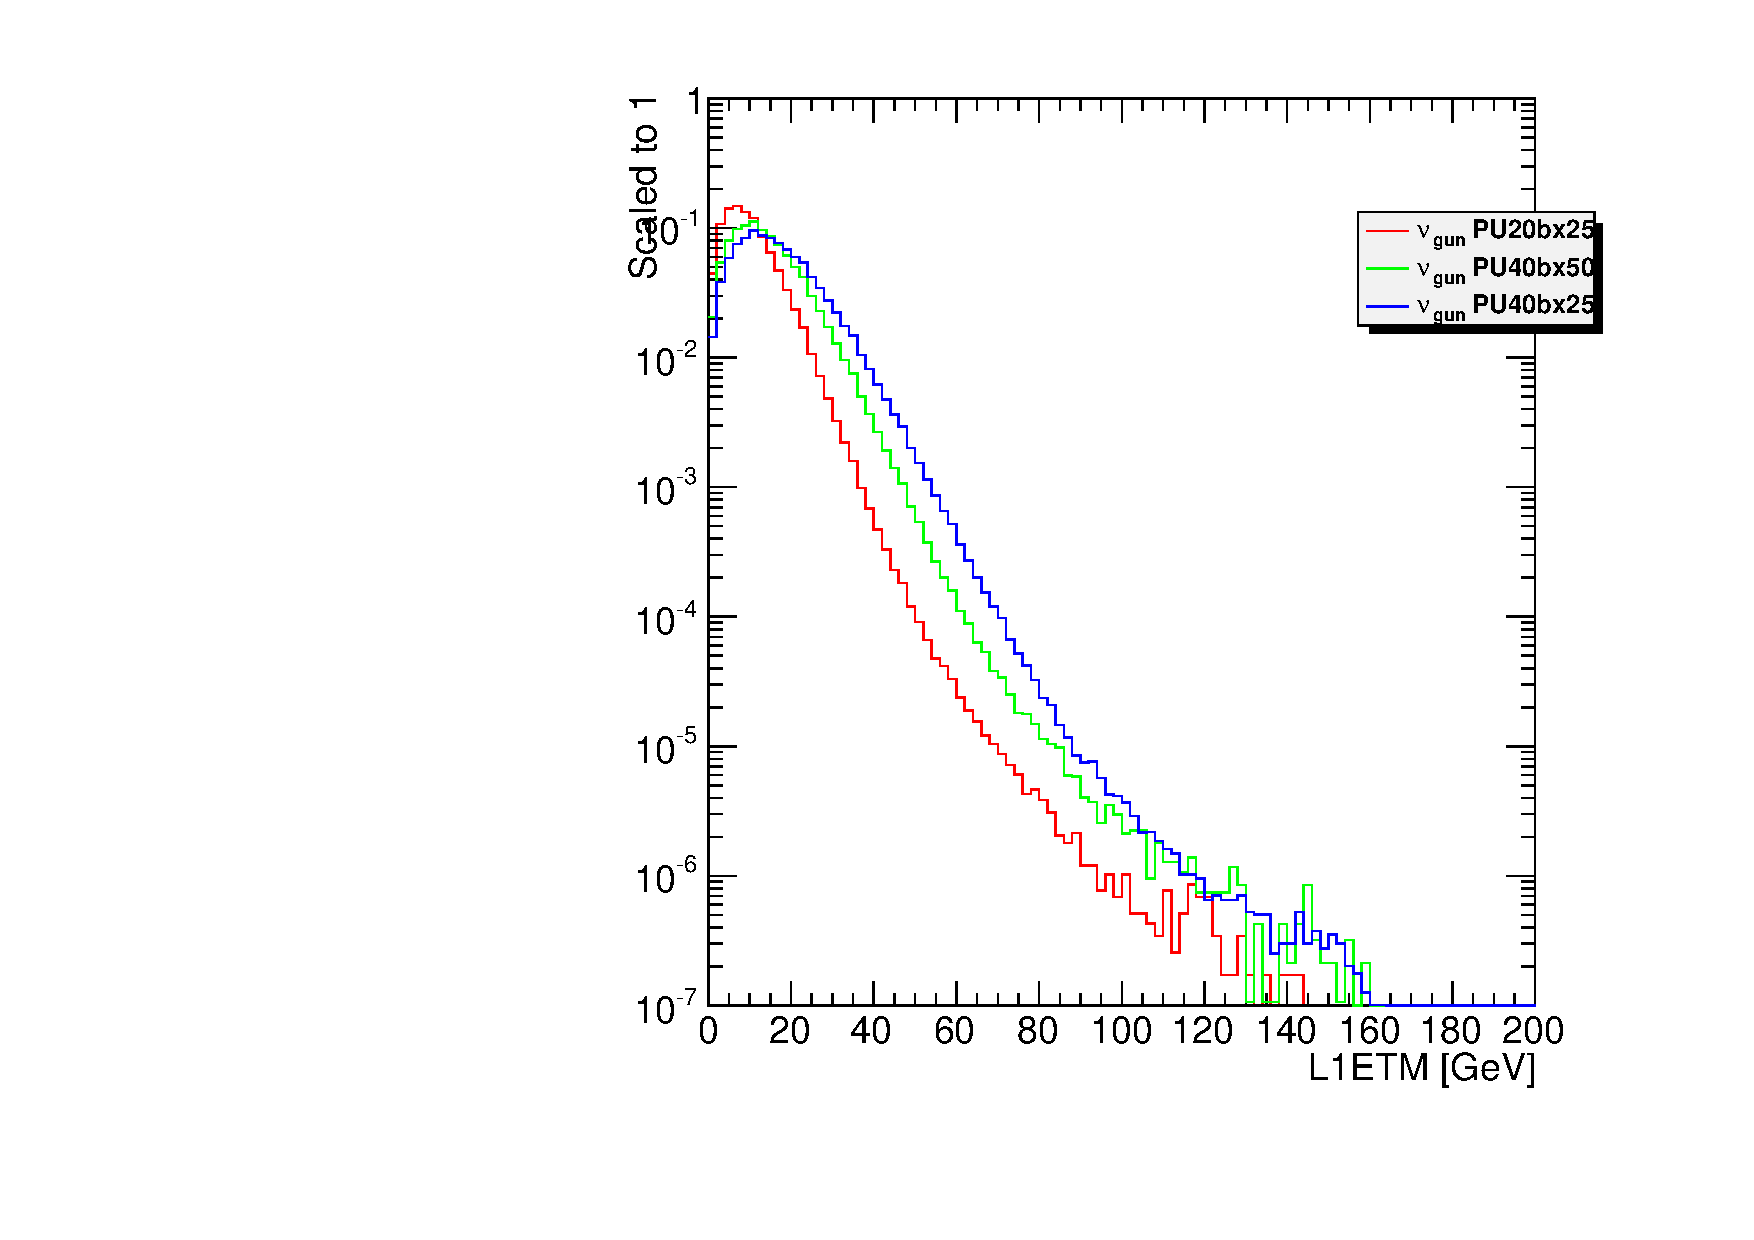
\includegraphics[width=\linewidth]{fig/L1ETM_NG.pdf}
 
\end{block}

\column[t]{0.45\linewidth}
\begin{block}{L1T HTT}
 
\centering
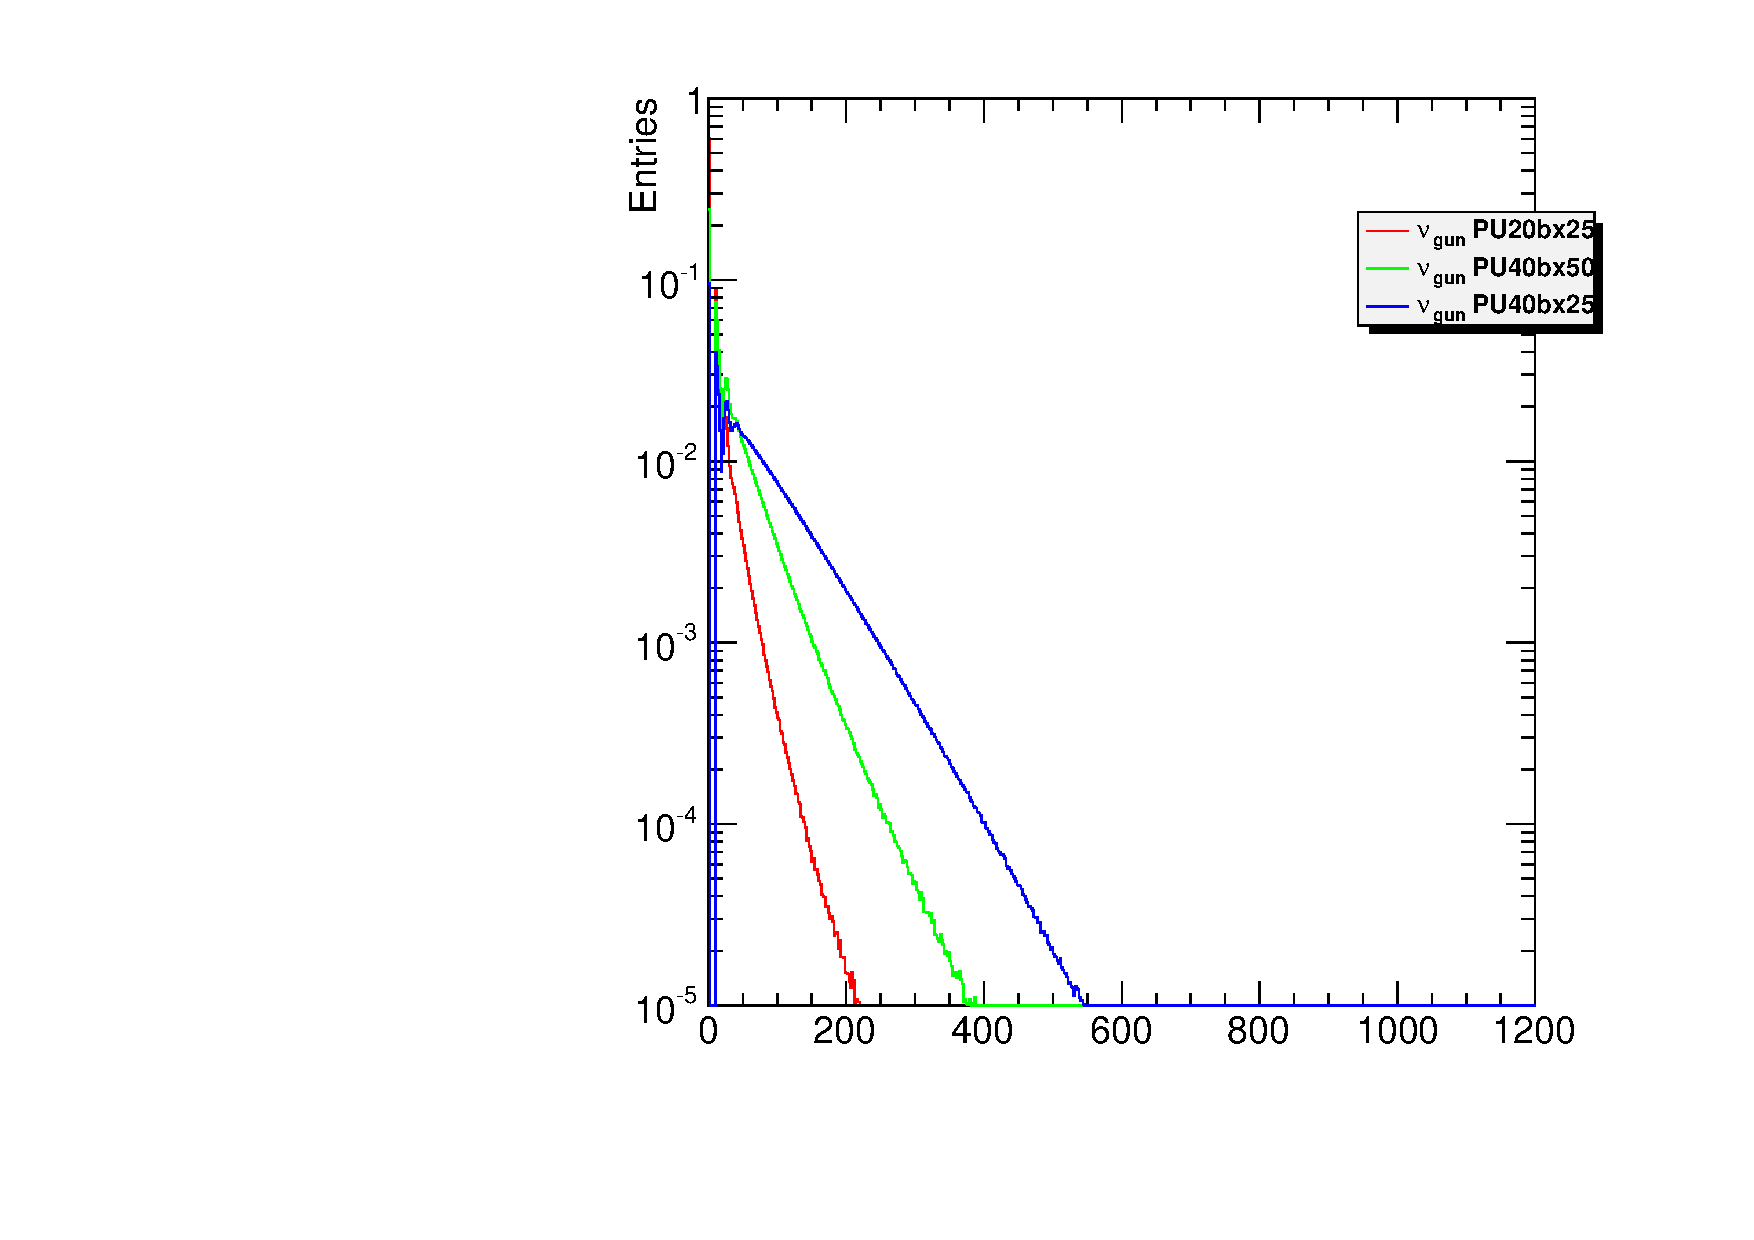
\includegraphics[width=\linewidth]{fig/L1HTT_NG.pdf}
 
\end{block}

\end{columns}

As expected with increasing PU and decreasing separation, is is more likely to get higher of getting ETM and HTT. Still ETM seams less affected then HTT. 

\end{frame}

% ###################################################
\begin{frame}{Neutrino Gun - Efficiency per bunch}

\begin{columns}

\column[t]{0.40\linewidth}
\begin{block}{L1T}
\centering

\resizebox{1.0\linewidth}{!}{

\begin{tabular}{|c||c|c|c|}
\hline
L1T & PU20bx25 & PU40bx50 & PU40bx25 \\
\hline \hline
L1\_ETM30 & 0.010483 & 0.048612 & 0.099152 \\
L1\_ETM36 & 0.003418 & 0.018527 & 0.044528 \\
L1\_ETM40 & 0.001750 & 0.009856 & 0.025847 \\
L1\_ETM50 & 0.000418 & 0.002087 & 0.006257 \\
L1\_ETM70 & 0.000058 & 0.000194 & 0.000427 \\
L1\_ETM100 & 0.000009 & 0.000023 & 0.000028 \\
L1\_HTT150 & 0.001237 & 0.024361 & 0.136941 \\
L1\_HTT175 & 0.000645 & 0.014350 & 0.095888 \\
L1\_HTT200 & 0.000349 & 0.008607 & 0.066854 \\
\hline
\end{tabular}


}

\end{block}

\column[t]{0.55\linewidth}
\begin{block}{Notes}
 
\begin{itemize}
  \item We can see that going from L1\_ETM40 to L1\_ETM70 reduced significantly the amount of event passing (more than a factor 30)
  \item Again we see a strange effects on the efficiency of parked VBF HLT Paths
  \item We can separate by seed to try to disentangle.
\end{itemize}
 
\end{block}

\end{columns}

\begin{block}{HLT (Just for indicative purposes)}
\centering
 
\resizebox{0.8\linewidth}{!}{ 
\begin{tabular}{|c||c|c|c|}
\hline
HLT & PU20bx25 & PU40bx50 & PU40bx25 \\
\hline \hline
HLT\_DiPFJet40\_PFMETnoMu65\_MJJ800VBF\_AllJets\_v & 0.000002 & 0.000008 & 0.000034 \\
HLT\_DiPFJet40\_PFMETnoMu75\_MJJ800VBF\_AllJets\_v & 0.000002 & 0.000006 & 0.000025 \\
HLT\_DiPFJet40\_PFMETnoMu65\_MJJ600VBF\_LeadingJets\_v & 0.000004 & 0.000012 & 0.000060 \\
HLT\_DiPFJet40\_PFMETnoMu75\_MJJ600VBF\_LeadingJets\_v & 0.000002 & 0.000008 & 0.000046 \\
HLT\_DiJet20\_MJJ650\_AllJets\_DEta3p5\_HT120\_VBF\_v & 0.000140 & 0.000422 & 0.000247 \\
HLT\_DiJet30\_MJJ700\_AllJets\_DEta3p5\_VBF\_v & 0.000094 & 0.000238 & 0.000118 \\
HLT\_DiJet35\_MJJ650\_AllJets\_DEta3p5\_VBF\_v & 0.000095 & 0.000224 & 0.000132 \\
HLT\_DiJet35\_MJJ700\_AllJets\_DEta3p5\_VBF\_v & 0.000077 & 0.000176 & 0.000093 \\
HLT\_DiJet35\_MJJ750\_AllJets\_DEta3p5\_VBF\_v & 0.000064 & 0.000148 & 0.000072 \\
\hline
\end{tabular}

 }

\end{block}

\end{frame}

% ###################################################
\begin{frame}{Neutrino Gun - Efficiency per bunch per seed (\% of total) I}

\begin{columns}

\column[t]{0.50\linewidth}
\begin{block}{HLT - ETM Seed only}
\centering

\resizebox{1.0\linewidth}{!}{ 
\begin{tabular}{|c||c|c|c|}
\hline
HLT & PU20bx25 & PU40bx50 & PU40bx25 \\
\hline \hline
HLT\_DiPFJet40\_PFMETnoMu65\_MJJ800VBF\_AllJets\_v & 1.000000 & 1.000000 & 1.000000 \\
HLT\_DiPFJet40\_PFMETnoMu75\_MJJ800VBF\_AllJets\_v & 1.000000 & 1.000000 & 1.000000 \\
HLT\_DiPFJet40\_PFMETnoMu65\_MJJ600VBF\_LeadingJets\_v & 1.000000 & 1.000000 & 1.000000 \\
HLT\_DiPFJet40\_PFMETnoMu75\_MJJ600VBF\_LeadingJets\_v & 1.000000 & 1.000000 & 1.000000 \\
HLT\_DiJet20\_MJJ650\_AllJets\_DEta3p5\_HT120\_VBF\_v & 0.690012 & 0.416898 & 0.354374 \\
HLT\_DiJet30\_MJJ700\_AllJets\_DEta3p5\_VBF\_v & 0.703839 & 0.518568 & 0.347299 \\
HLT\_DiJet35\_MJJ650\_AllJets\_DEta3p5\_VBF\_v & 0.540395 & 0.375059 & 0.222709 \\
HLT\_DiJet35\_MJJ700\_AllJets\_DEta3p5\_VBF\_v & 0.680045 & 0.496372 & 0.317571 \\
HLT\_DiJet35\_MJJ750\_AllJets\_DEta3p5\_VBF\_v & 0.660027 & 0.514039 & 0.320958 \\
\hline
\end{tabular}

 }

\end{block}

\begin{block}{HLT - HTT Seed only}
\centering
 
\resizebox{1.0\linewidth}{!}{ 
\begin{tabular}{|c||c|c|c|}
\hline
HLT & PU20bx25 & PU40bx50 & PU40bx25 \\
\hline \hline
HLT\_DiPFJet40\_PFMETnoMu65\_MJJ800VBF\_AllJets\_v & 0.000000 & 0.000000 & 0.000000 \\
HLT\_DiPFJet40\_PFMETnoMu75\_MJJ800VBF\_AllJets\_v & 0.000000 & 0.000000 & 0.000000 \\
HLT\_DiPFJet40\_PFMETnoMu65\_MJJ600VBF\_LeadingJets\_v & 0.000000 & 0.000000 & 0.000000 \\
HLT\_DiPFJet40\_PFMETnoMu75\_MJJ600VBF\_LeadingJets\_v & 0.000000 & 0.000000 & 0.000000 \\
HLT\_DiJet20\_MJJ650\_AllJets\_DEta3p5\_HT120\_VBF\_v & 0.176614 & 0.361160 & 0.319160 \\
HLT\_DiJet30\_MJJ700\_AllJets\_DEta3p5\_VBF\_v & 0.160878 & 0.244295 & 0.266695 \\
HLT\_DiJet35\_MJJ650\_AllJets\_DEta3p5\_VBF\_v & 0.238779 & 0.300333 & 0.317775 \\
HLT\_DiJet35\_MJJ700\_AllJets\_DEta3p5\_VBF\_v & 0.175028 & 0.227328 & 0.261956 \\
HLT\_DiJet35\_MJJ750\_AllJets\_DEta3p5\_VBF\_v & 0.187251 & 0.215983 & 0.258501 \\
\hline
\end{tabular}

 }

\end{block}

\begin{block}{HLT - Both ETM and HTT Seeds}
\centering

\resizebox{1.0\linewidth}{!}{ 
\begin{tabular}{|c||c|c|c|}
\hline
HLT & PU20bx25 & PU40bx50 & PU40bx25 \\
\hline \hline
HLT\_DiPFJet40\_PFMETnoMu65\_MJJ800VBF\_AllJets\_v & 0.000000 & 0.000000 & 0.000000 \\
HLT\_DiPFJet40\_PFMETnoMu75\_MJJ800VBF\_AllJets\_v & 0.000000 & 0.000000 & 0.000000 \\
HLT\_DiPFJet40\_PFMETnoMu65\_MJJ600VBF\_LeadingJets\_v & 0.000000 & 0.000000 & 0.000000 \\
HLT\_DiPFJet40\_PFMETnoMu75\_MJJ600VBF\_LeadingJets\_v & 0.000000 & 0.000000 & 0.000000 \\
HLT\_DiJet20\_MJJ650\_AllJets\_DEta3p5\_HT120\_VBF\_v & 0.133374 & 0.221942 & 0.326466 \\
HLT\_DiJet30\_MJJ700\_AllJets\_DEta3p5\_VBF\_v & 0.135283 & 0.237136 & 0.386006 \\
HLT\_DiJet35\_MJJ650\_AllJets\_DEta3p5\_VBF\_v & 0.220826 & 0.324607 & 0.459516 \\
HLT\_DiJet35\_MJJ700\_AllJets\_DEta3p5\_VBF\_v & 0.144928 & 0.276300 & 0.420473 \\
HLT\_DiJet35\_MJJ750\_AllJets\_DEta3p5\_VBF\_v & 0.152722 & 0.269978 & 0.420541 \\
\hline
\end{tabular}

 }

\end{block}

\column[t]{0.40\linewidth}
\begin{block}{Notes:}
\centering

\begin{itemize}
  \item It looks like as we go move up in scenario:
  \begin{itemize}
    \item L1\_ETM only seed percentage goes down
    \item L1\_HTT only goes up from PU20bx25 to PU40bx50 but does not change much to PU40bx25
    \item Bith L1\_ETM and L1\_HTT goes up 
  \end{itemize}
  \item So it looks that the global behavior comes from the different trends of the seed components 
\end{itemize}

\end{block}

\end{columns}

\end{frame}

% ###################################################
\begin{frame}{Neutrino Gun - Efficiency per bunch per seed (\% of total) II}

Here is an illustration to show what happens:

\begin{columns}
\column[t]{0.47\linewidth}
\begin{block}{\footnotesize HLT\_DiJet20\_MJJ650\_AllJets\_DEta3p5\_HT120\_VBF\_v}
 
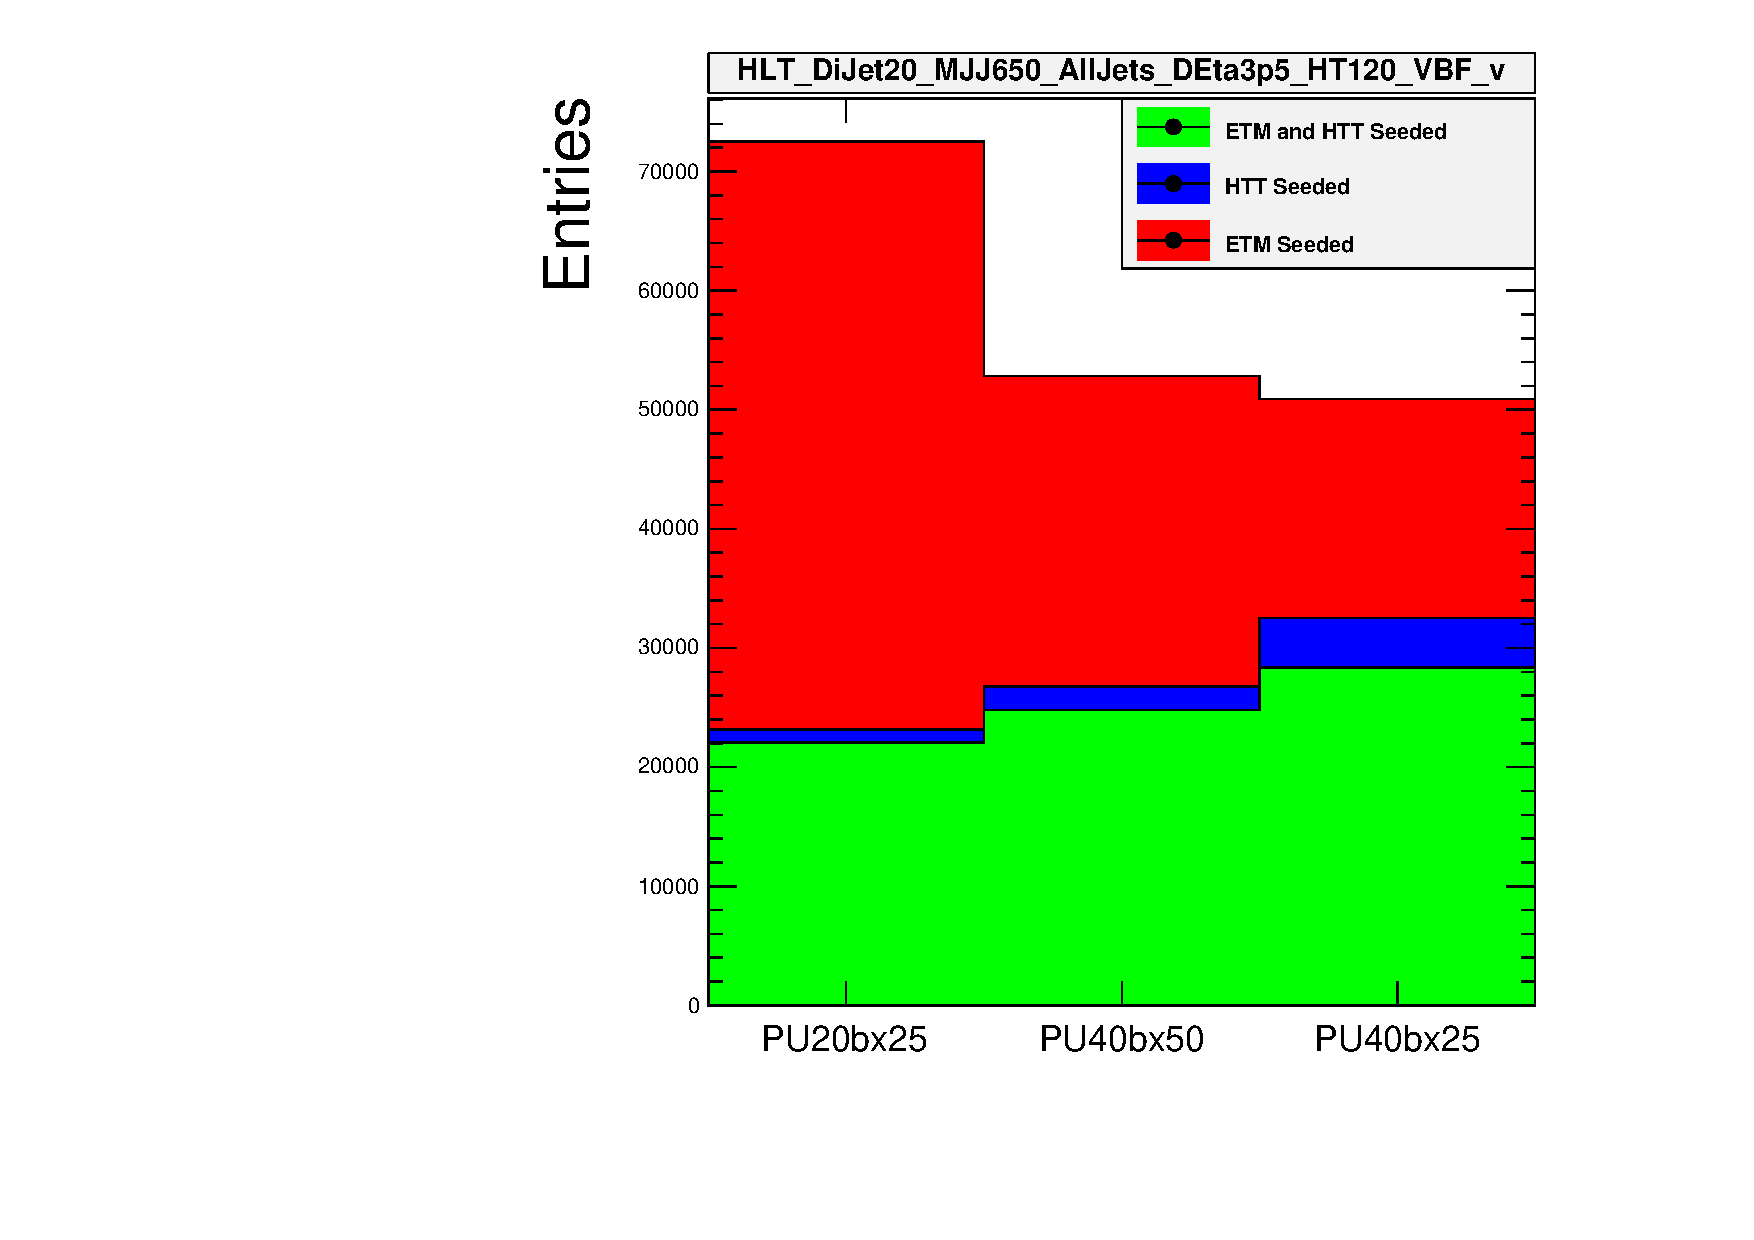
\includegraphics[width=\linewidth]{fig/HLT_DiJet20_MJJ650_AllJets_DEta3p5_HT120_VBF_v.pdf}

\end{block}

\column[t]{0.47\linewidth}
\begin{block}{\footnotesize HLT\_DiJet35\_MJJ650\_AllJets\_DEta3p5\_VBF\_v}
 
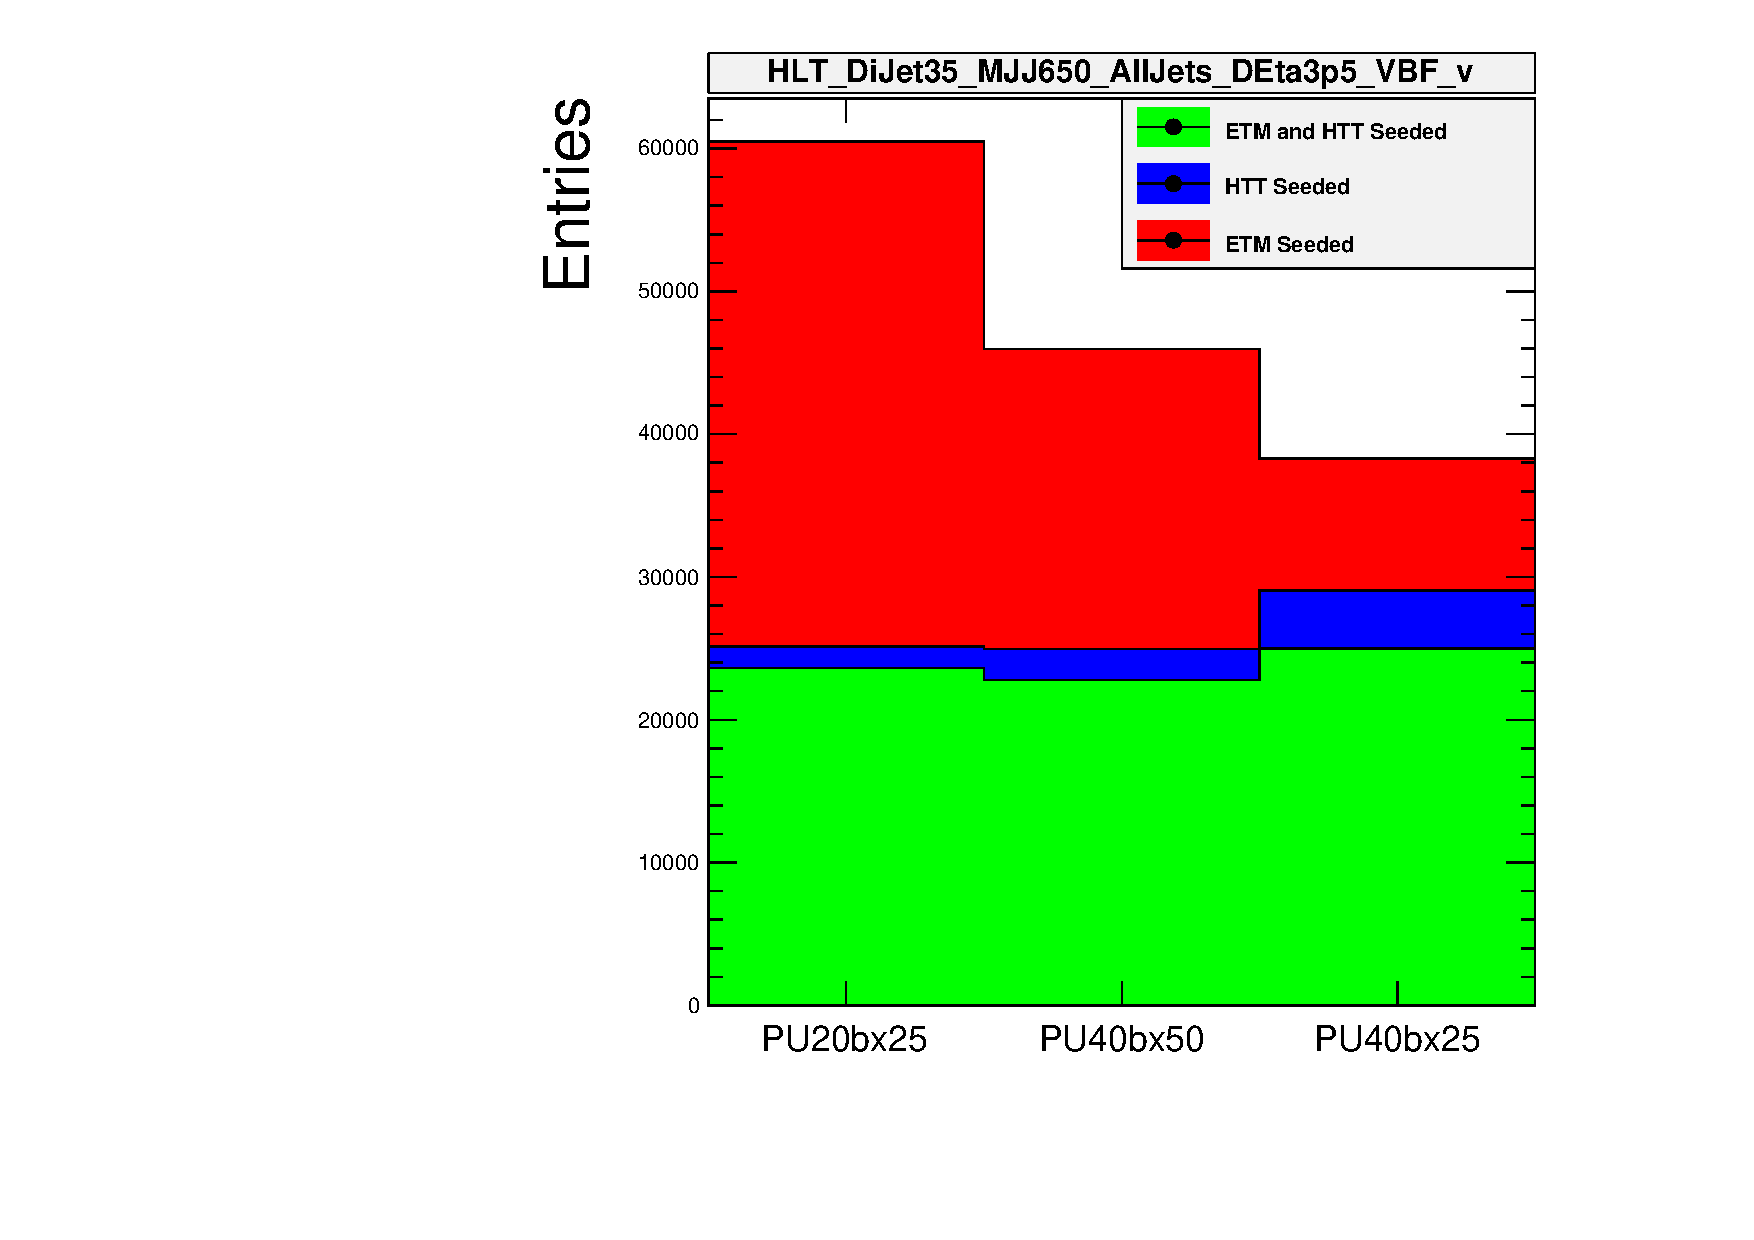
\includegraphics[width=\linewidth]{fig/HLT_DiJet35_MJJ650_AllJets_DEta3p5_VBF_v.pdf}
 
\end{block}

\end{columns}

This shows that the global trend is in fact dominated by the decrease in efficiency of L1\_ETM seeds. Other parked triggers plots at backup slides.

\end{frame}

% ###################################################
\begin{frame}{Neutrino Gun - Rate per bunch}

\begin{columns}

\column[t]{0.40\linewidth}
\begin{block}{L1T}
\centering

\resizebox{1.0\linewidth}{!}{

\begin{tabular}{|c||c|c|c|}
\hline
L1T & PU20bx25 & PU40bx50 & PU40bx25 \\
\hline \hline
L1\_ETM30 & 117.886507 & 546.690500 & 1115.065568 \\
L1\_ETM36 & 38.441378 & 208.359154 & 500.764801 \\
L1\_ETM40 & 19.675335 & 110.841428 & 290.679881 \\
L1\_ETM50 & 4.701373 & 23.475891 & 70.363804 \\
L1\_ETM70 & 0.648532 & 2.176153 & 4.799886 \\
L1\_ETM100 & 0.101032 & 0.263196 & 0.309625 \\
L1\_HTT150 & 13.911678 & 273.965555 & 1540.037268 \\
L1\_HTT175 & 7.251238 & 161.375070 & 1078.359393 \\
L1\_HTT200 & 3.929679 & 96.799919 & 751.844350 \\
\hline
\end{tabular}


}

\end{block}

\column[t]{0.55\linewidth}
\begin{block}{Notes}
 
\begin{itemize}
  \item Here we just apply the neutrino gun efficiency to the rate per bunch
\end{itemize}
 
\end{block}

\end{columns}

\begin{block}{HLT (Just for indicative purposes)}
\centering
 
\resizebox{0.8\linewidth}{!}{ 
\begin{tabular}{|c||c|c|c|}
\hline
HLT & PU20bx25 & PU40bx50 & PU40bx25 \\
\hline \hline
HLT\_DiPFJet40\_PFMETnoMu65\_MJJ800VBF\_AllJets\_v & 0.027904 & 0.092119 & 0.385831 \\
HLT\_DiPFJet40\_PFMETnoMu75\_MJJ800VBF\_AllJets\_v & 0.019244 & 0.062210 & 0.285916 \\
HLT\_DiPFJet40\_PFMETnoMu65\_MJJ600VBF\_LeadingJets\_v & 0.040413 & 0.130402 & 0.674852 \\
HLT\_DiPFJet40\_PFMETnoMu75\_MJJ600VBF\_LeadingJets\_v & 0.023093 & 0.088530 & 0.517923 \\
HLT\_DiJet20\_MJJ650\_AllJets\_DEta3p5\_HT120\_VBF\_v & 1.579954 & 4.743511 & 2.781258 \\
HLT\_DiJet30\_MJJ700\_AllJets\_DEta3p5\_VBF\_v & 1.052661 & 2.673833 & 1.327124 \\
HLT\_DiJet35\_MJJ650\_AllJets\_DEta3p5\_VBF\_v & 1.071905 & 2.513522 & 1.481513 \\
HLT\_DiJet35\_MJJ700\_AllJets\_DEta3p5\_VBF\_v & 0.863105 & 1.978756 & 1.050522 \\
HLT\_DiJet35\_MJJ750\_AllJets\_DEta3p5\_VBF\_v & 0.724547 & 1.661724 & 0.813435 \\
\hline
\end{tabular}

 }

\end{block}

\end{frame}

% ###################################################
\begin{frame}{Neutrino Gun - Maximum Pure Rate}

\begin{columns}

\column[t]{0.40\linewidth}
\begin{block}{L1T}
\centering

\resizebox{1.0\linewidth}{!}{

\begin{tabular}{|c||c|c|c|}
\hline
L1T & PU20bx25 & PU40bx50 & PU40bx25 \\
\hline \hline
L1\_ETM30 & 331025.311467 & 754432.890247 & 3131104.113764 \\
L1\_ETM36 & 107943.388769 & 287535.632691 & 1406147.559908 \\
L1\_ETM40 & 55248.339555 & 152961.170678 & 816229.106391 \\
L1\_ETM50 & 13201.456723 & 32396.730191 & 197581.560547 \\
L1\_ETM70 & 1821.076920 & 3003.090874 & 13478.080613 \\
L1\_ETM100 & 283.698927 & 363.210551 & 869.425758 \\
L1\_HTT150 & 39063.991260 & 378072.466354 & 4324424.649249 \\
L1\_HTT175 & 20361.477254 & 222697.596469 & 3028033.175055 \\
L1\_HTT200 & 11034.537302 & 133583.887783 & 2111178.934776 \\
\hline
\end{tabular}


}

\end{block}

\column[t]{0.55\linewidth}
\begin{block}{Notes}
 
\begin{itemize}
  \item We can now apply the maximum number of bunch for each configuration which is 2808 for 25 ns and 1380 for 50 ns and calculate maximum pure 
  \item As seen before the rates explode the unmanageable values.
\end{itemize}
 
\end{block}

\end{columns}

\begin{block}{HLT}
\centering

\resizebox{0.8\linewidth}{!}{
\begin{tabular}{|c||c|c|c|}
\hline
HLT & PU20bx25 & PU40bx50 & PU40bx25 \\
\hline \hline
HLT\_DiPFJet40\_PFMETnoMu65\_MJJ800VBF\_AllJets\_v & 78.354942 & 127.123693 & 1083.413866 \\
HLT\_DiPFJet40\_PFMETnoMu75\_MJJ800VBF\_AllJets\_v & 54.037891 & 85.849767 & 802.851679 \\
HLT\_DiPFJet40\_PFMETnoMu65\_MJJ600VBF\_LeadingJets\_v & 113.479571 & 179.954318 & 1894.983579 \\
HLT\_DiPFJet40\_PFMETnoMu75\_MJJ600VBF\_LeadingJets\_v & 64.845469 & 122.170822 & 1454.326586 \\
HLT\_DiJet20\_MJJ650\_AllJets\_DEta3p5\_HT120\_VBF\_v & 4436.510835 & 6546.044703 & 7809.773395 \\
HLT\_DiJet30\_MJJ700\_AllJets\_DEta3p5\_VBF\_v & 2955.872627 & 3689.889007 & 3726.563274 \\
HLT\_DiJet35\_MJJ650\_AllJets\_DEta3p5\_VBF\_v & 3009.910518 & 3468.660762 & 4160.087330 \\
HLT\_DiJet35\_MJJ700\_AllJets\_DEta3p5\_VBF\_v & 2423.599402 & 2730.682961 & 2949.865697 \\
HLT\_DiJet35\_MJJ750\_AllJets\_DEta3p5\_VBF\_v & 2034.526589 & 2293.179342 & 2284.124916 \\
\hline
\end{tabular}

}

\end{block}

\end{frame}



% % ###################################################
% \begin{frame}{Understanding higher rates from 25 to 50 ns}
%  
% I have identified several possible reason for this higher rates
% \begin{block}{HLT}
%  
% \begin{itemize}
%   \item Higher out of time pile up (OOT PU) due to higher bunch density and bunch to bunch interaction which will add events to calorimeters
%   \item Saturation of ECAL or HCAL primitives and/or RCT zones
%   \item High integration times by HCAL or ECAL systems (more OOT PU recorded or even more bx) 
% \end{itemize}
% 
% \end{block}
%  
% Most like likely a combination of all of this effects.
%  
% \begin{block}{Steps taken}
%  
% \begin{itemize}
%   \item Contacted HCAL and Trigger Calorimeter experts and indeed we integrate for 50ns the energy so energy on the next event at 25 ns will be in pratice OOT PU always...
%   \item Recent studies have showed (see 2 weeks ago L1 DPG meeting) HCAL, ECAL or RCT saturation is now an issue and will generate ETM.
%   \item I am in contact with people upgrading algorithms so we can profit from this.
% \end{itemize}
% 
% \end{block} 
%  
% \end{frame}

\section{Trigger Tower and region saturation study}

% ###################################################
\begin{frame}{ECAL TT Compressed $E_{\perp}$}

Looking for ECAL TT saturation on Neutrino gun events and VBF H(inv) signal.

\begin{columns}
 
\column[t]{0.45\linewidth}
\begin{block}{Neutrino Gun - All events}
\centering

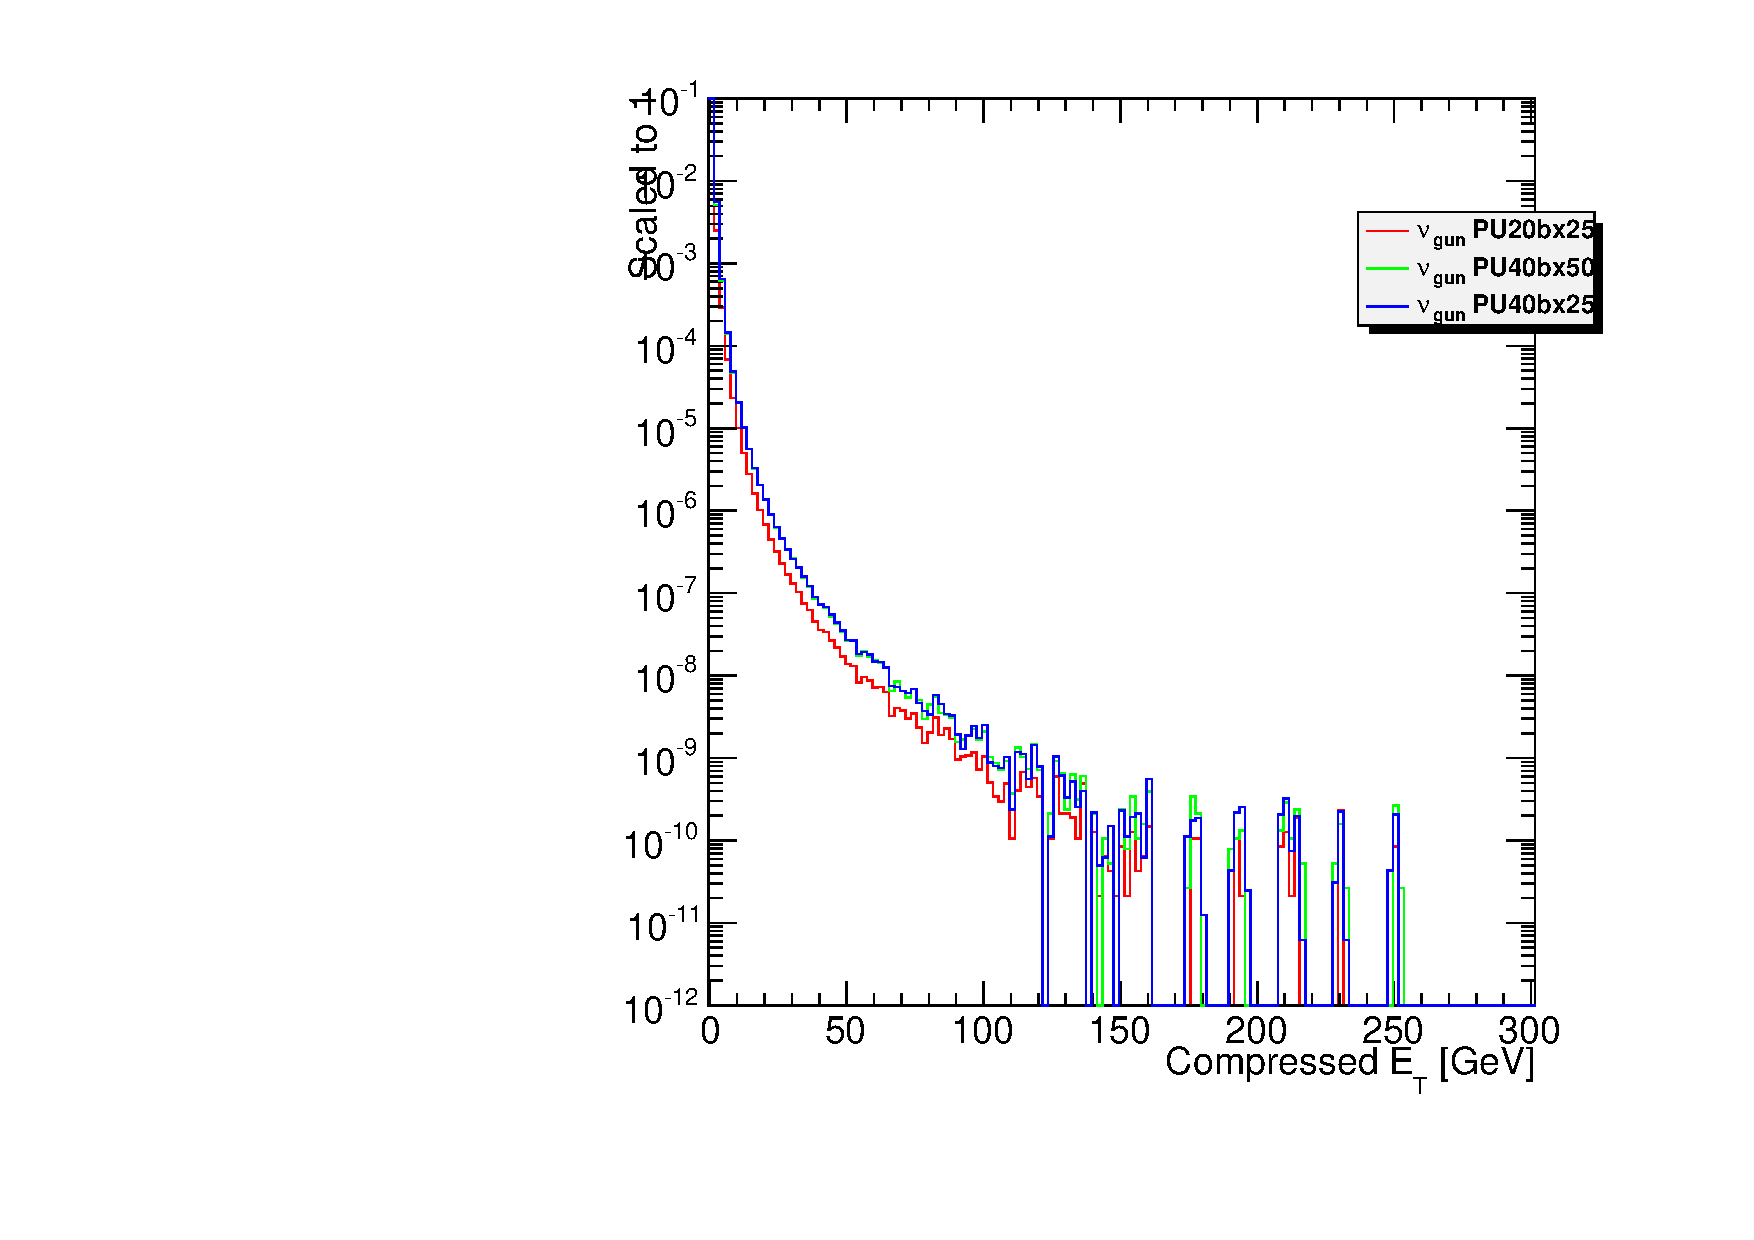
\includegraphics[width=\linewidth]{fig/EcalTT_Val_NG.pdf}

\end{block}

\column[t]{0.45\linewidth}
\begin{block}{VBF H(Inv) - All events}
\centering

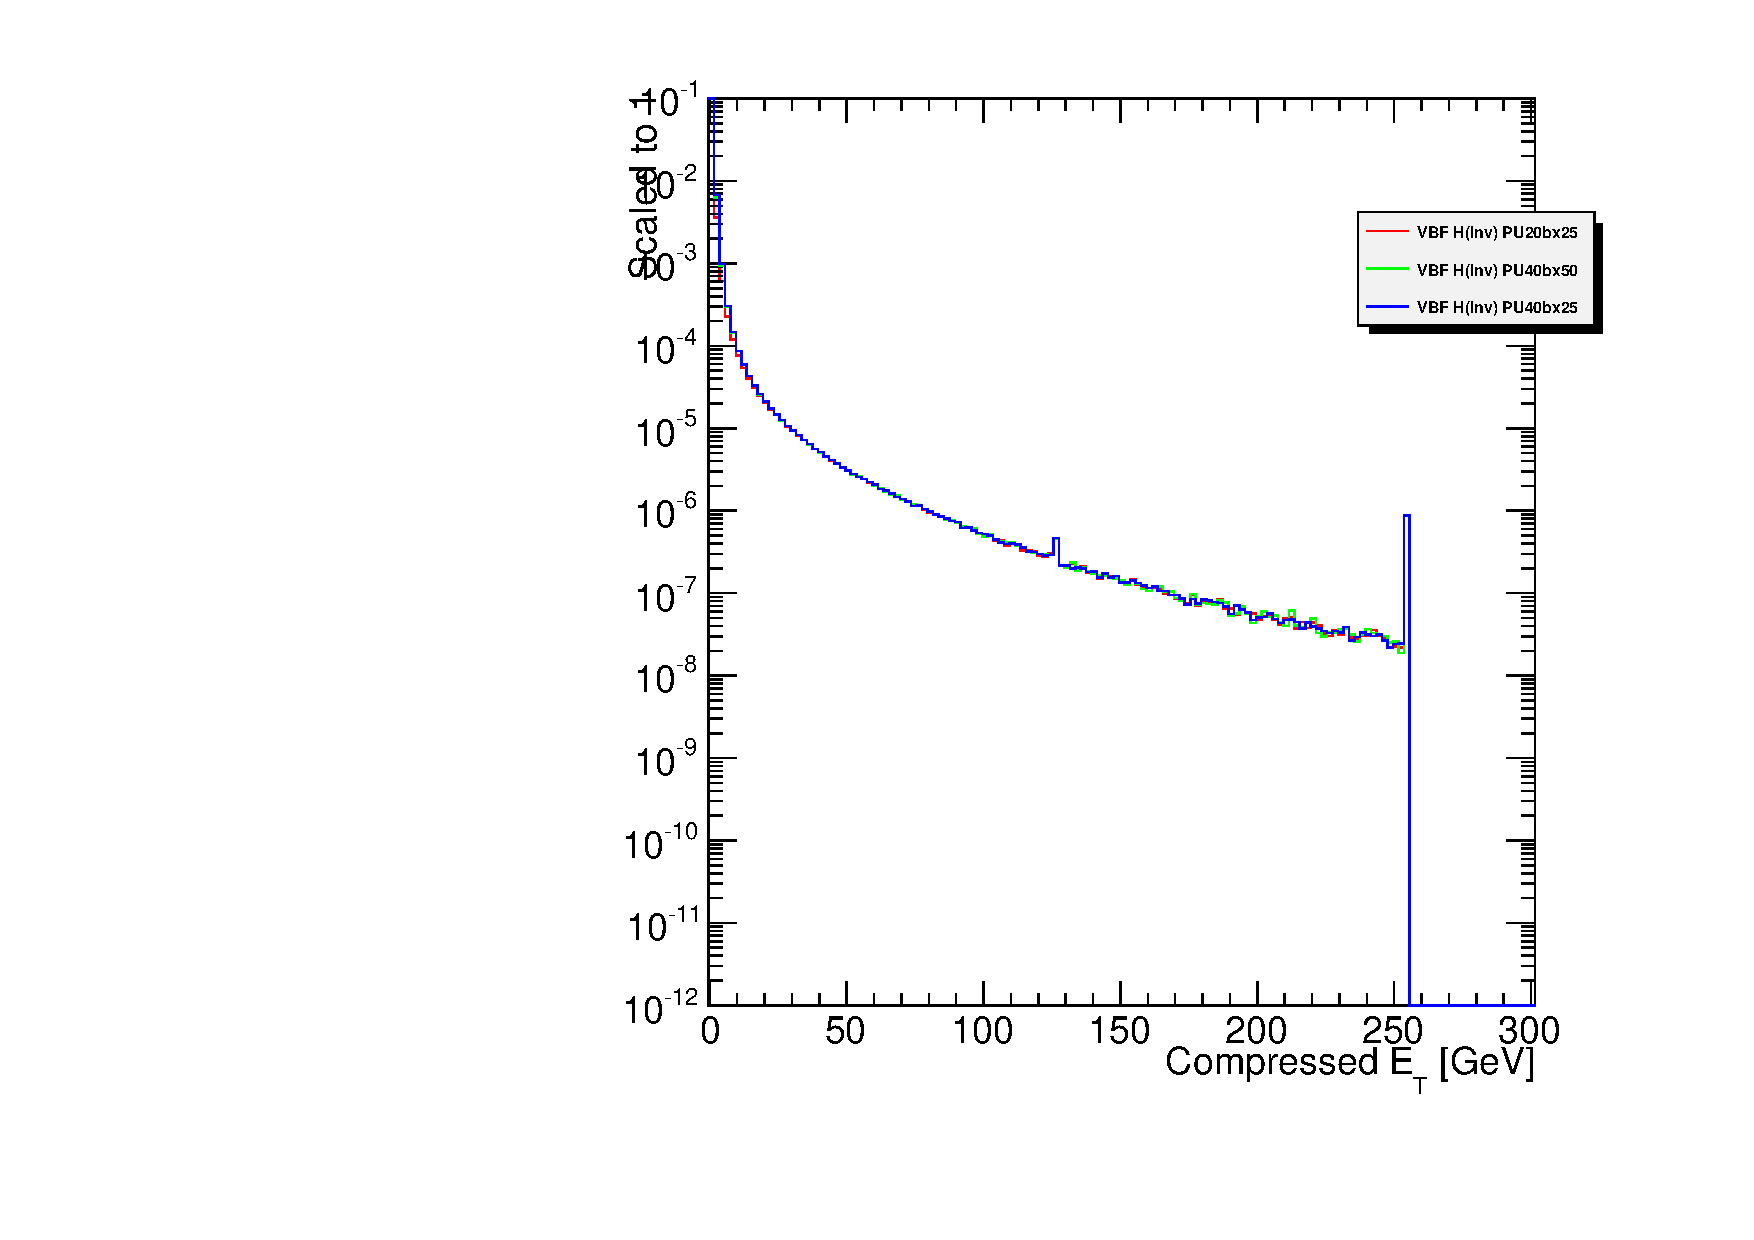
\includegraphics[width=\linewidth]{fig/EcalTT_Val_Sig.pdf}

\end{block}

\end{columns}

\begin{tiny}

\begin{itemize}
  \item ECAL TT saturation will not be a problem for us since is is an effect that cannot even be observed in neutrino gun samples.
  \item But we can clearly see saturation effects on our signal sample (much more energy available)
  \begin{itemize}
    \tiny
    \item The 255 peak is the expected saturation of 8 bit ECAL TT.
    \item As for 127 peak, after contacting several experts no one can really explain it!? 
  \end{itemize}
\end{itemize}

\end{tiny}

\end{frame}

% ###################################################
\begin{frame}{HCAL TT Compressed $E_{\perp}$}

Looking for HCAL TT saturation on Neutrino gun events and VBF H(inv) signal.

\begin{columns}
 
\column[t]{0.45\linewidth}
\begin{block}{Neutrino Gun - All events}
\centering

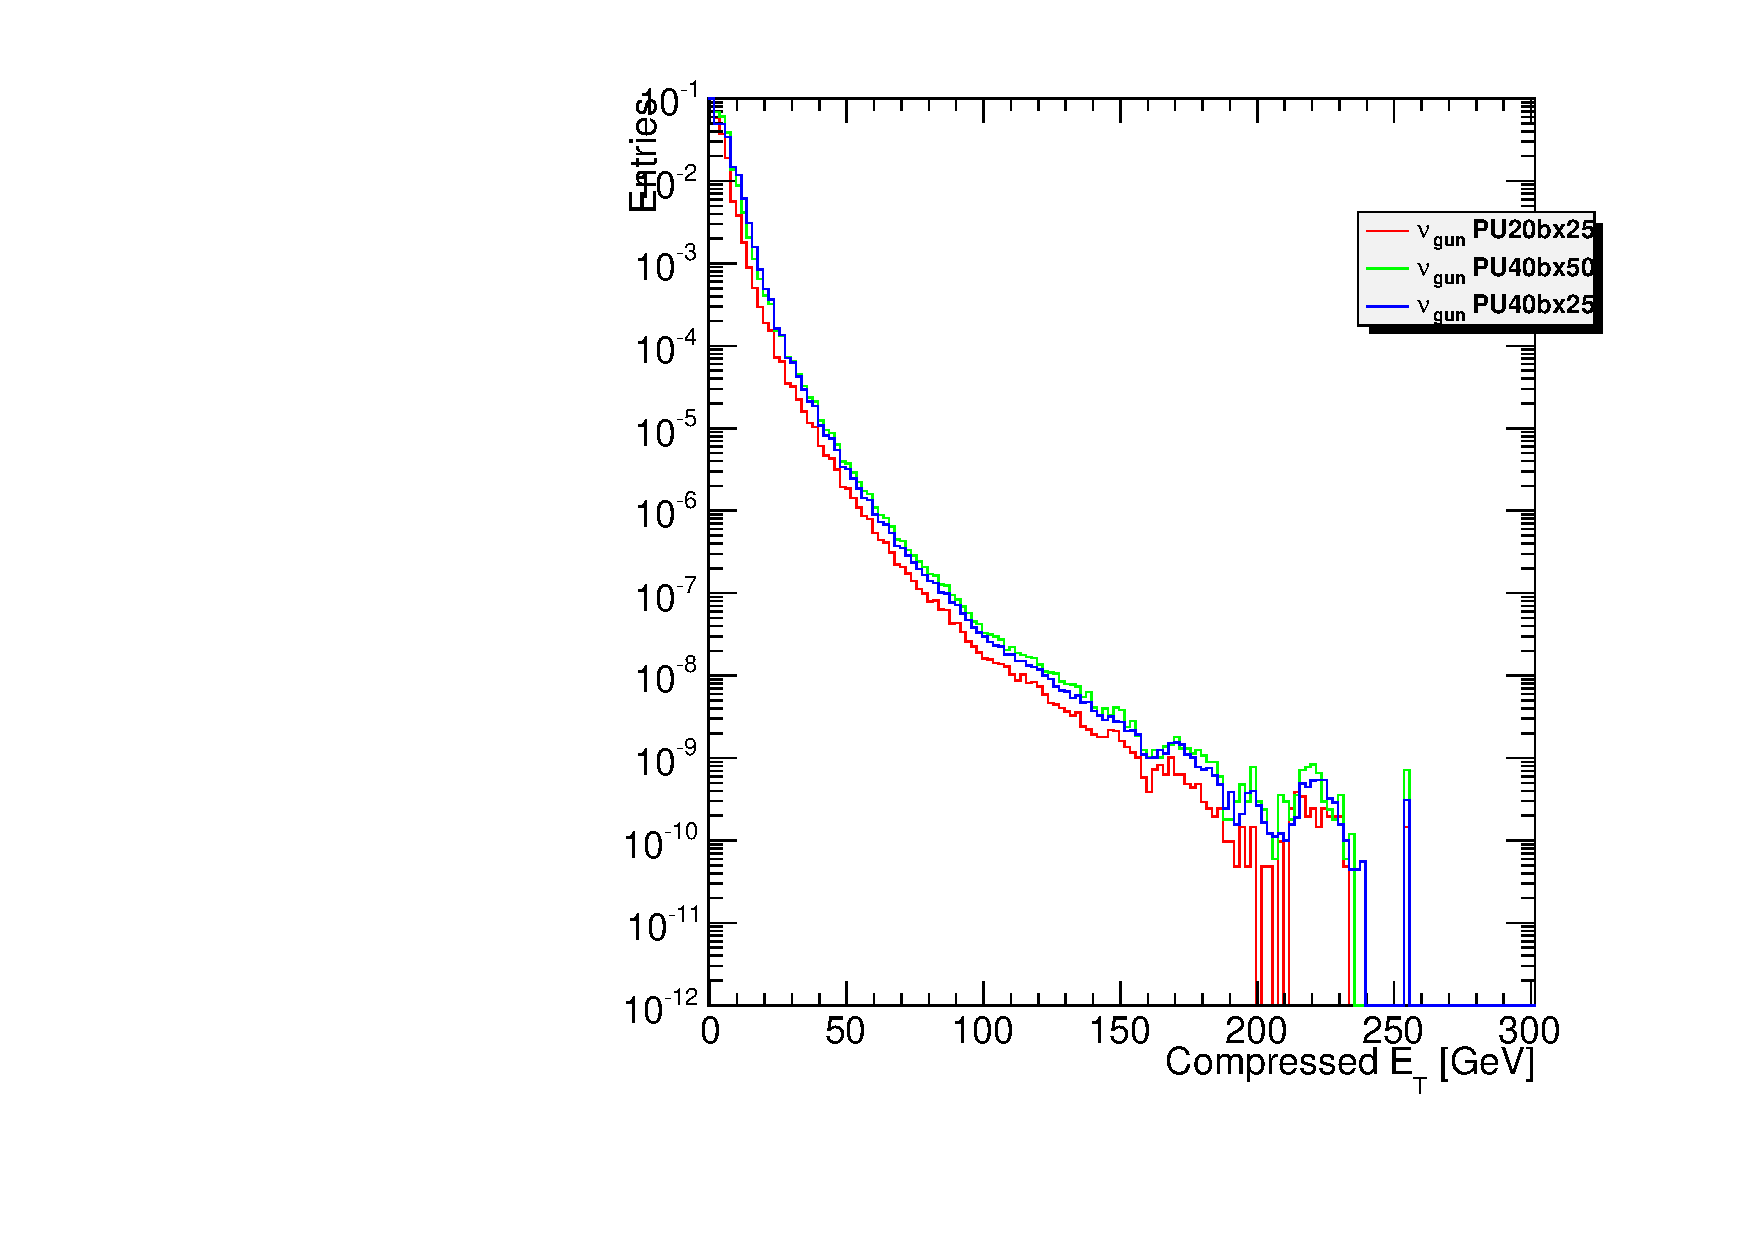
\includegraphics[width=\linewidth]{fig/HcalTT_Val_NG.pdf}

\end{block}

\column[t]{0.45\linewidth}
\begin{block}{VBF H(Inv) - All events}
\centering

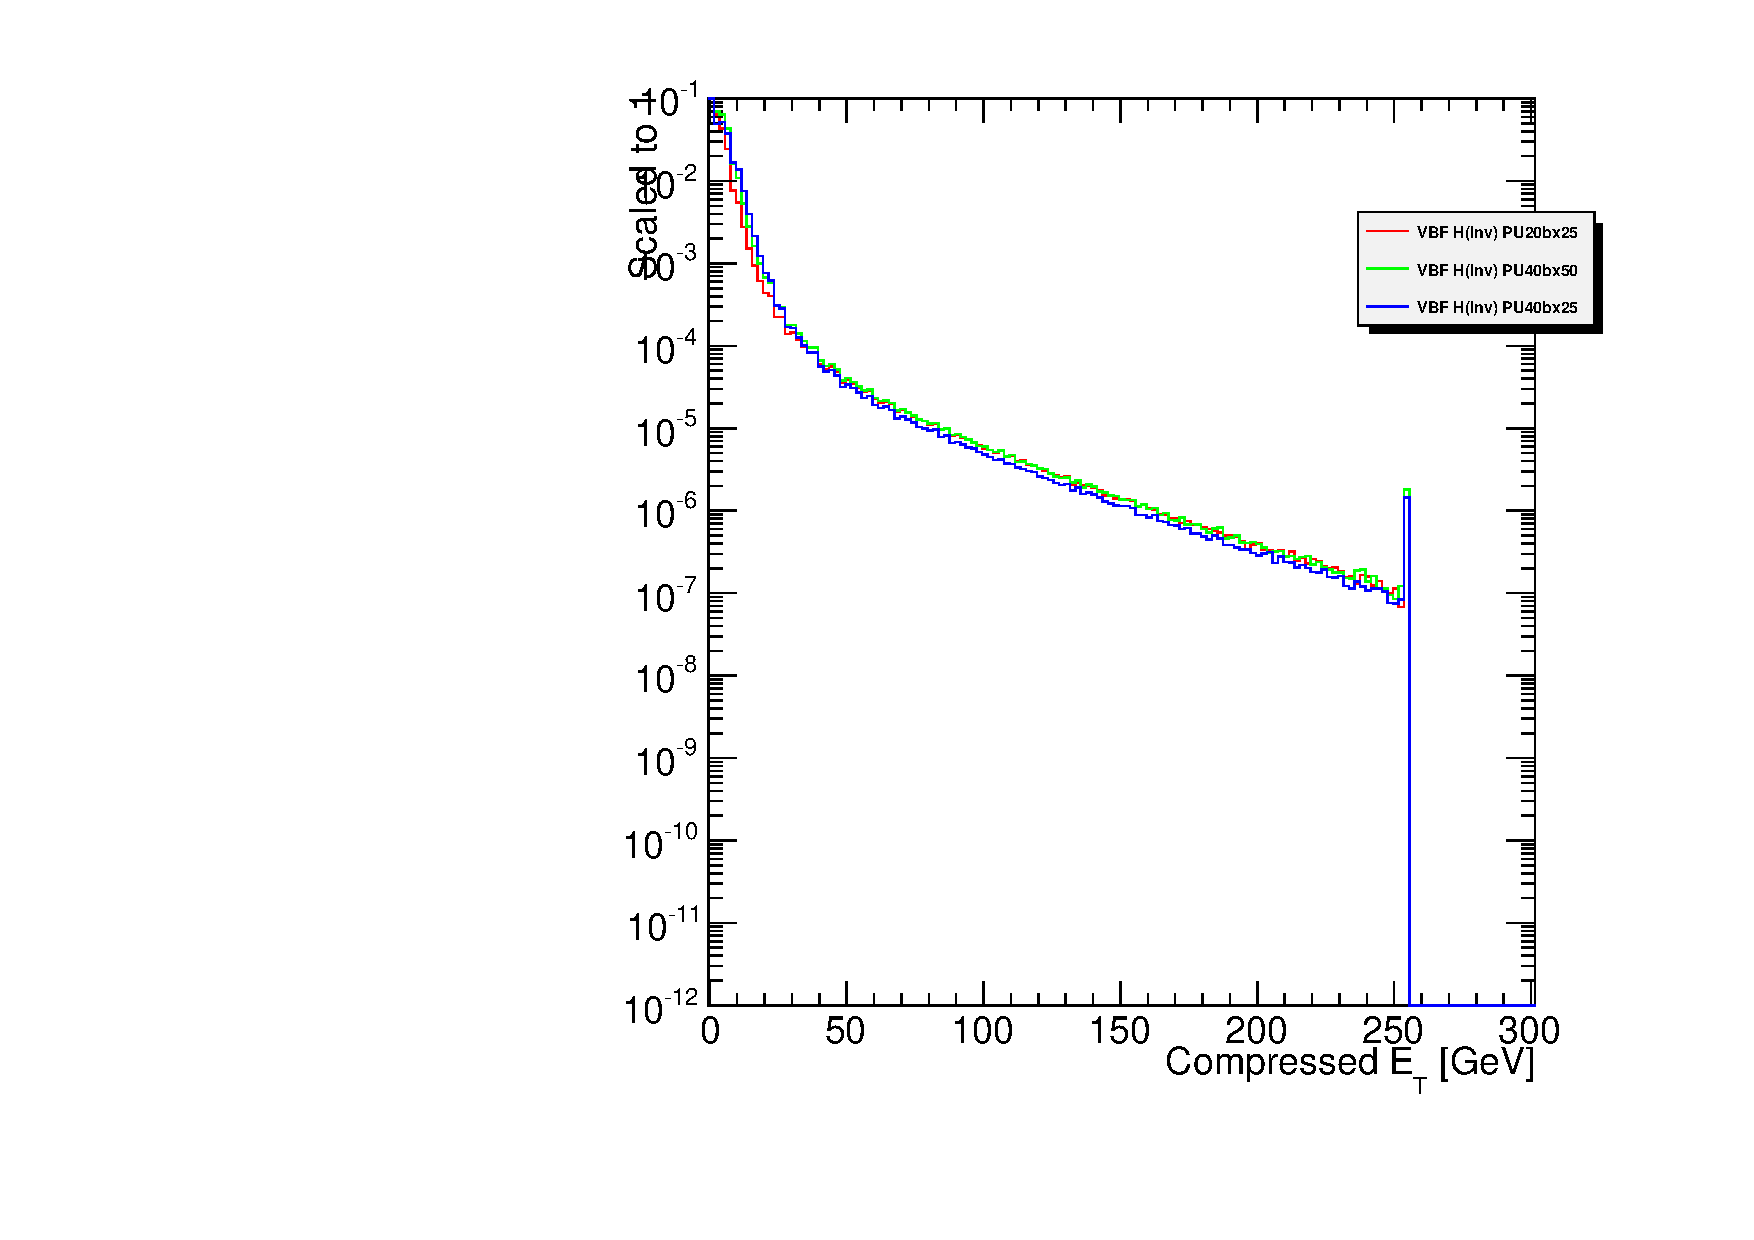
\includegraphics[width=\linewidth]{fig/HcalTT_Val_Sig.pdf}

\end{block}

\end{columns}

\begin{tiny}

\begin{itemize}
  \item HCAL TT saturation will not be a problem for us since is is an effect can barely be observed in neutrino gun samples.
  \item But we can clearly see saturation effects on our signal sample (much more energy available again) 
  \begin{itemize}
    \tiny
    \item The 255 peak is the expected saturation of 8 bit HCAL TT.
  \end{itemize}
\end{itemize}

\end{tiny}

\end{frame}

% ###################################################
\begin{frame}{RCT Region Compressed $E_{\perp}$}

Looking for RCT saturation on Neutrino gun events and VBF H(inv) signal.

\begin{columns}
 
\column[t]{0.45\linewidth}
\begin{block}{Neutrino Gun - All events}
\centering

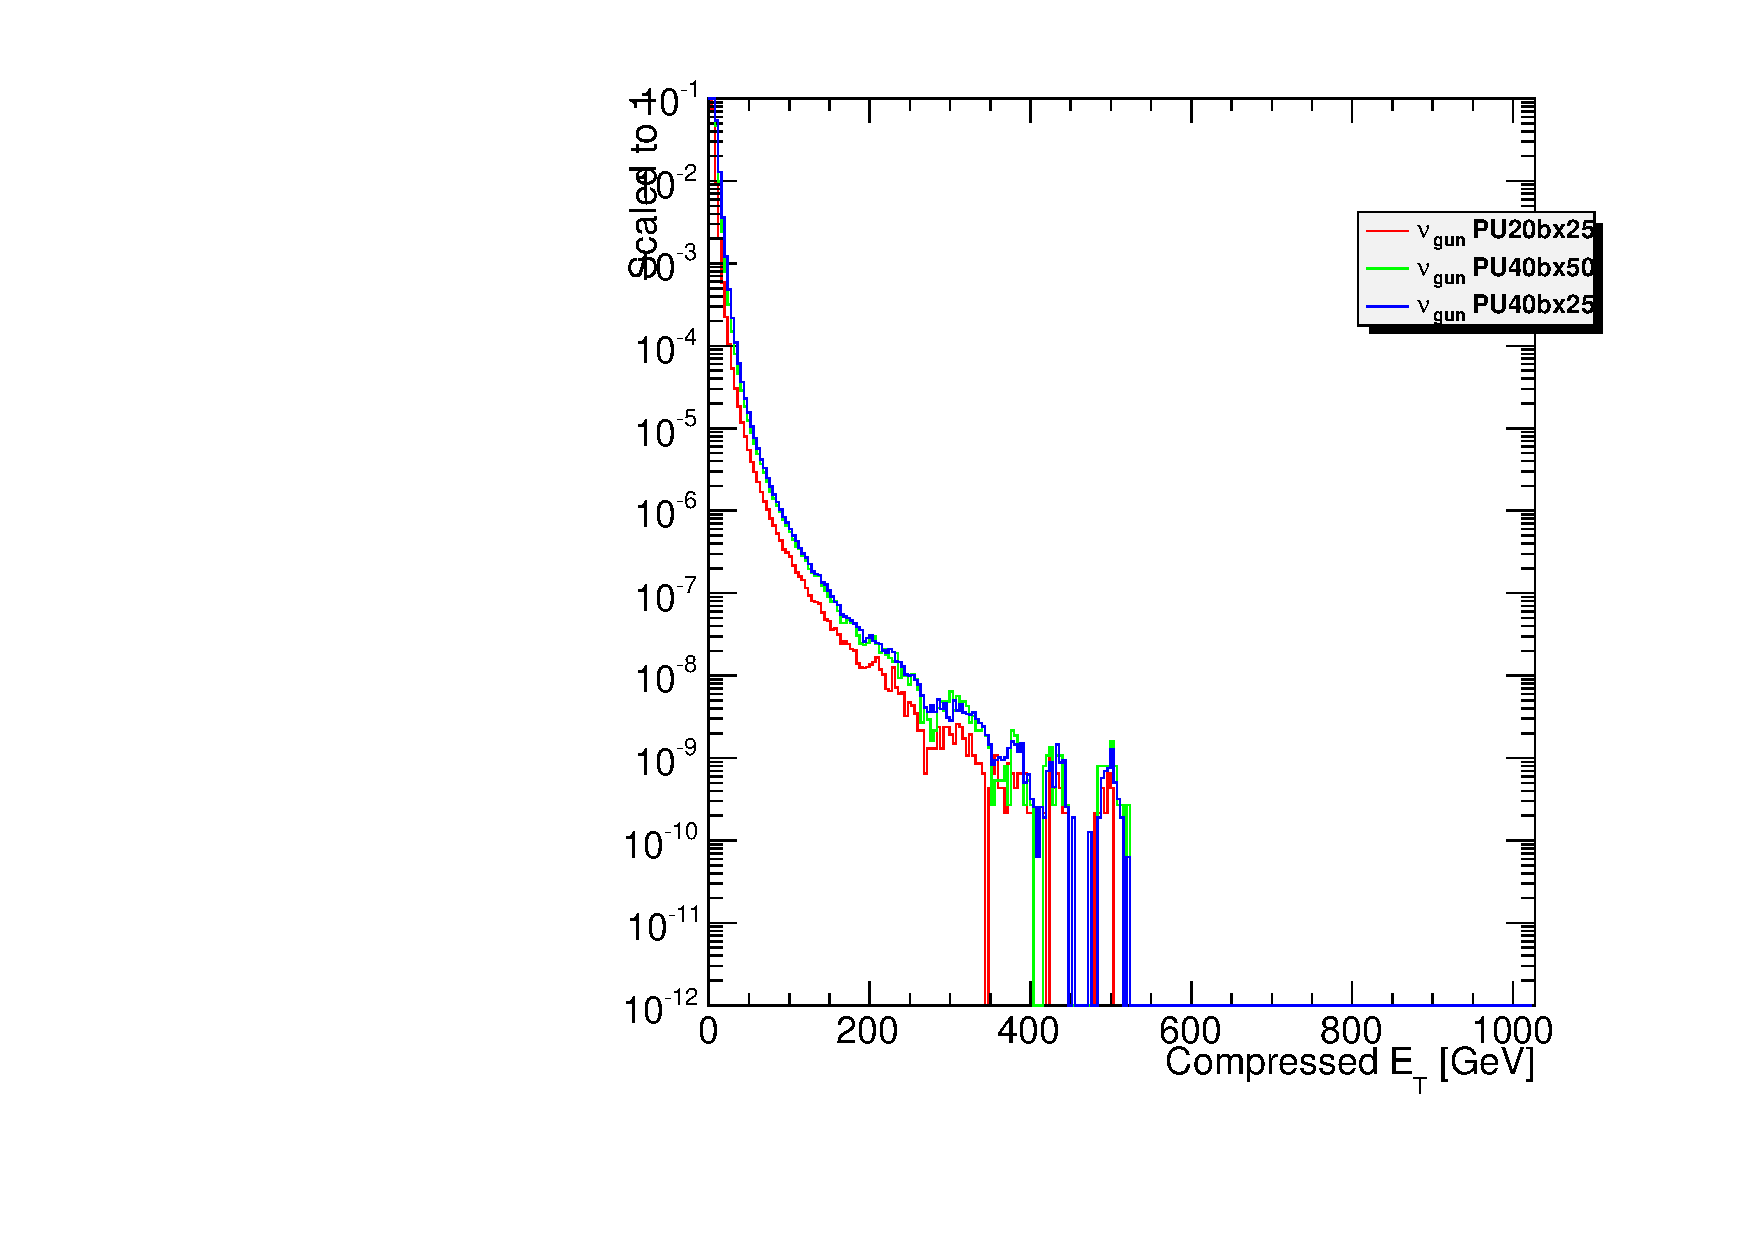
\includegraphics[width=\linewidth]{fig/RCTRegion_Val_NG.pdf}

\end{block}

\column[t]{0.45\linewidth}
\begin{block}{VBF H(Inv) - All events}
\centering

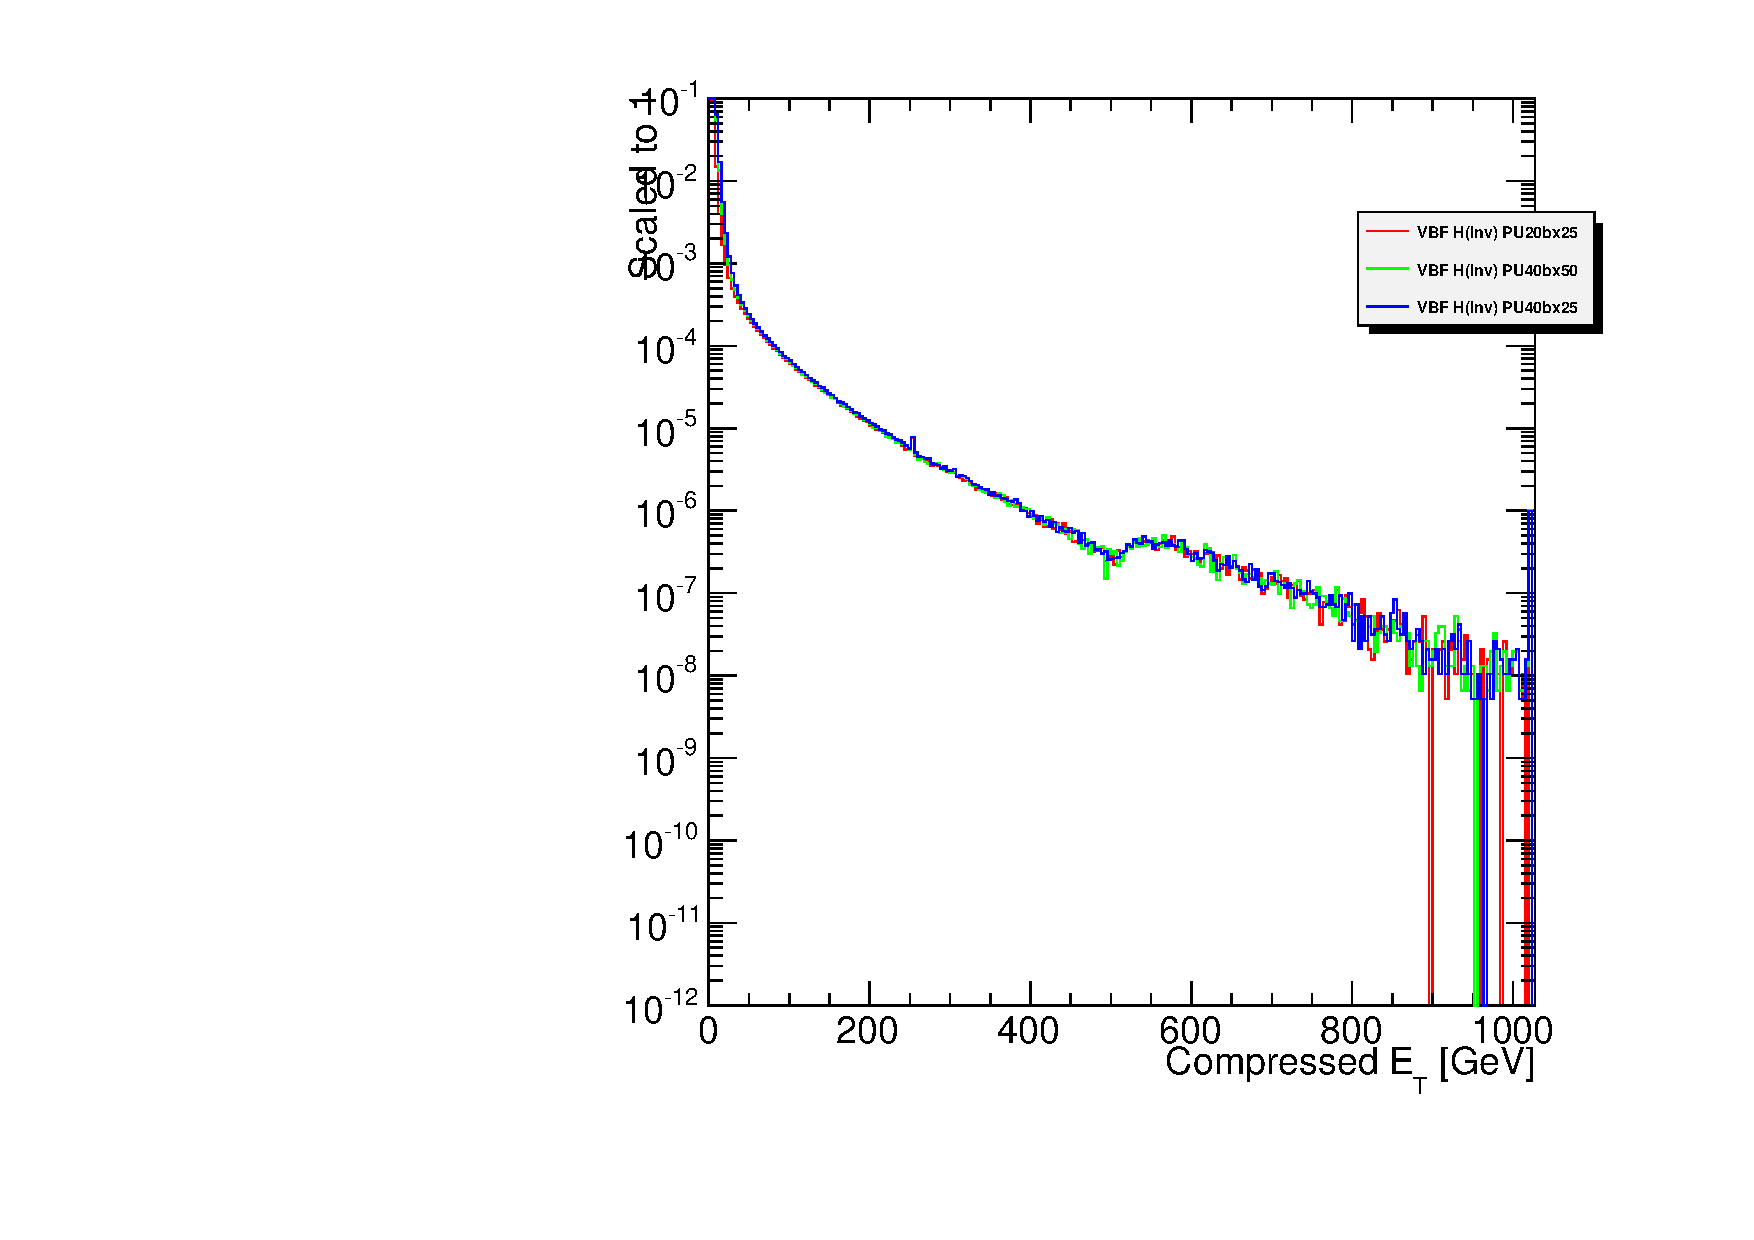
\includegraphics[width=\linewidth]{fig/RCTRegion_Val_Sig.pdf}

\end{block}

\end{columns}

\begin{tiny}

\begin{itemize}
  \item RCT Region saturation cannot also be observed on the neutrino gun so I think it will not be a problem.
  \item But we can clearly see saturation effects on our signal sample (much more energy available again) 
  \begin{itemize}
    \tiny
    \item The 255 peak is the expected saturation of 8 bit HCAL and ECAL TT.
    \item Above 511 we start seeing the effect of at least one RCT Region saturated. 
  \end{itemize}
\end{itemize}

\end{tiny}

\end{frame}

% ###################################################
\begin{frame}{Loking at ETM on saturated events I}

Now we can have a look at the properties of events of saturated ECAL TT (value=255), HCAL TT (value=255) or RCT Regions (value=511):

\begin{columns}
 
\column[t]{0.45\linewidth}
\begin{block}{VBF H(Inv) - All events}
\centering

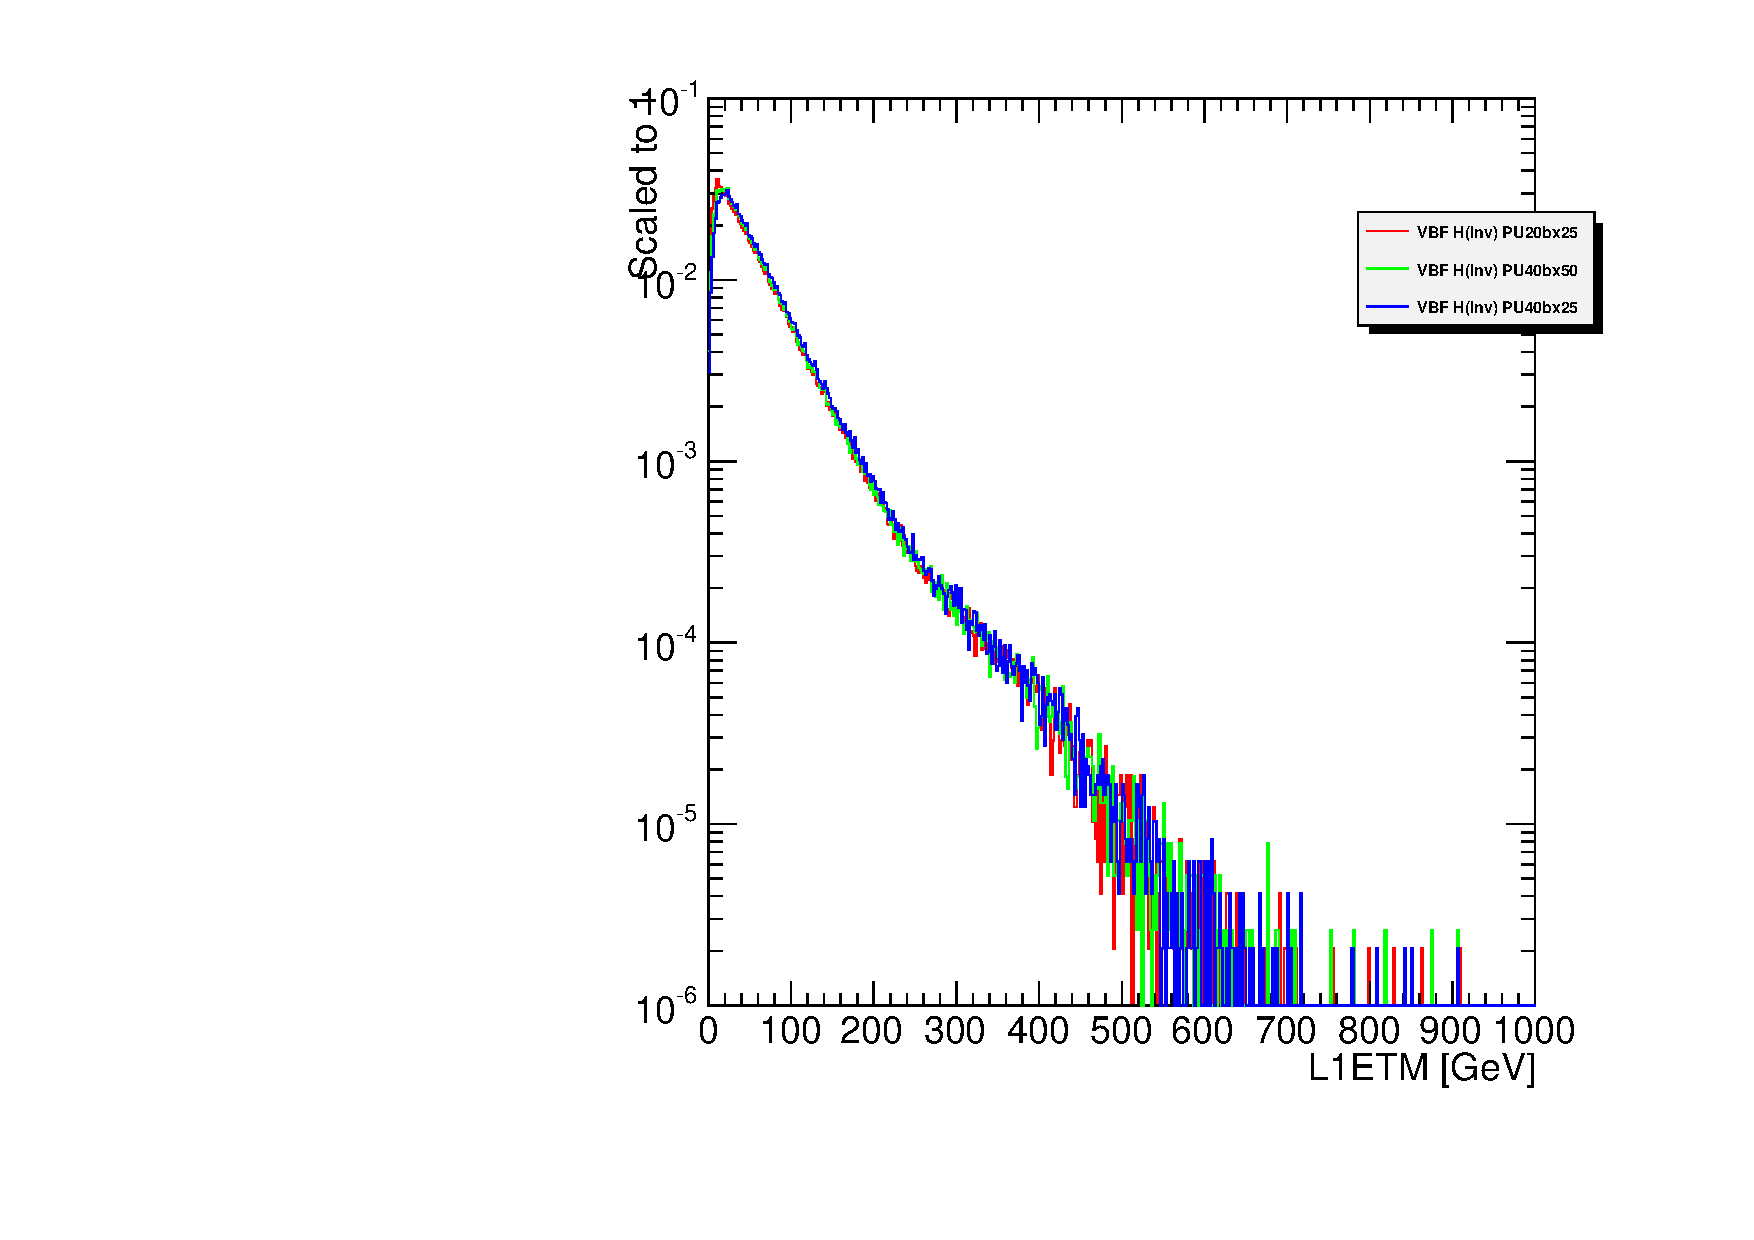
\includegraphics[width=\linewidth]{fig/L1ETM_Sig.pdf}

\end{block}

\column[t]{0.45\linewidth}
\begin{block}{VBF H(Inv) - Saturated events}
\centering

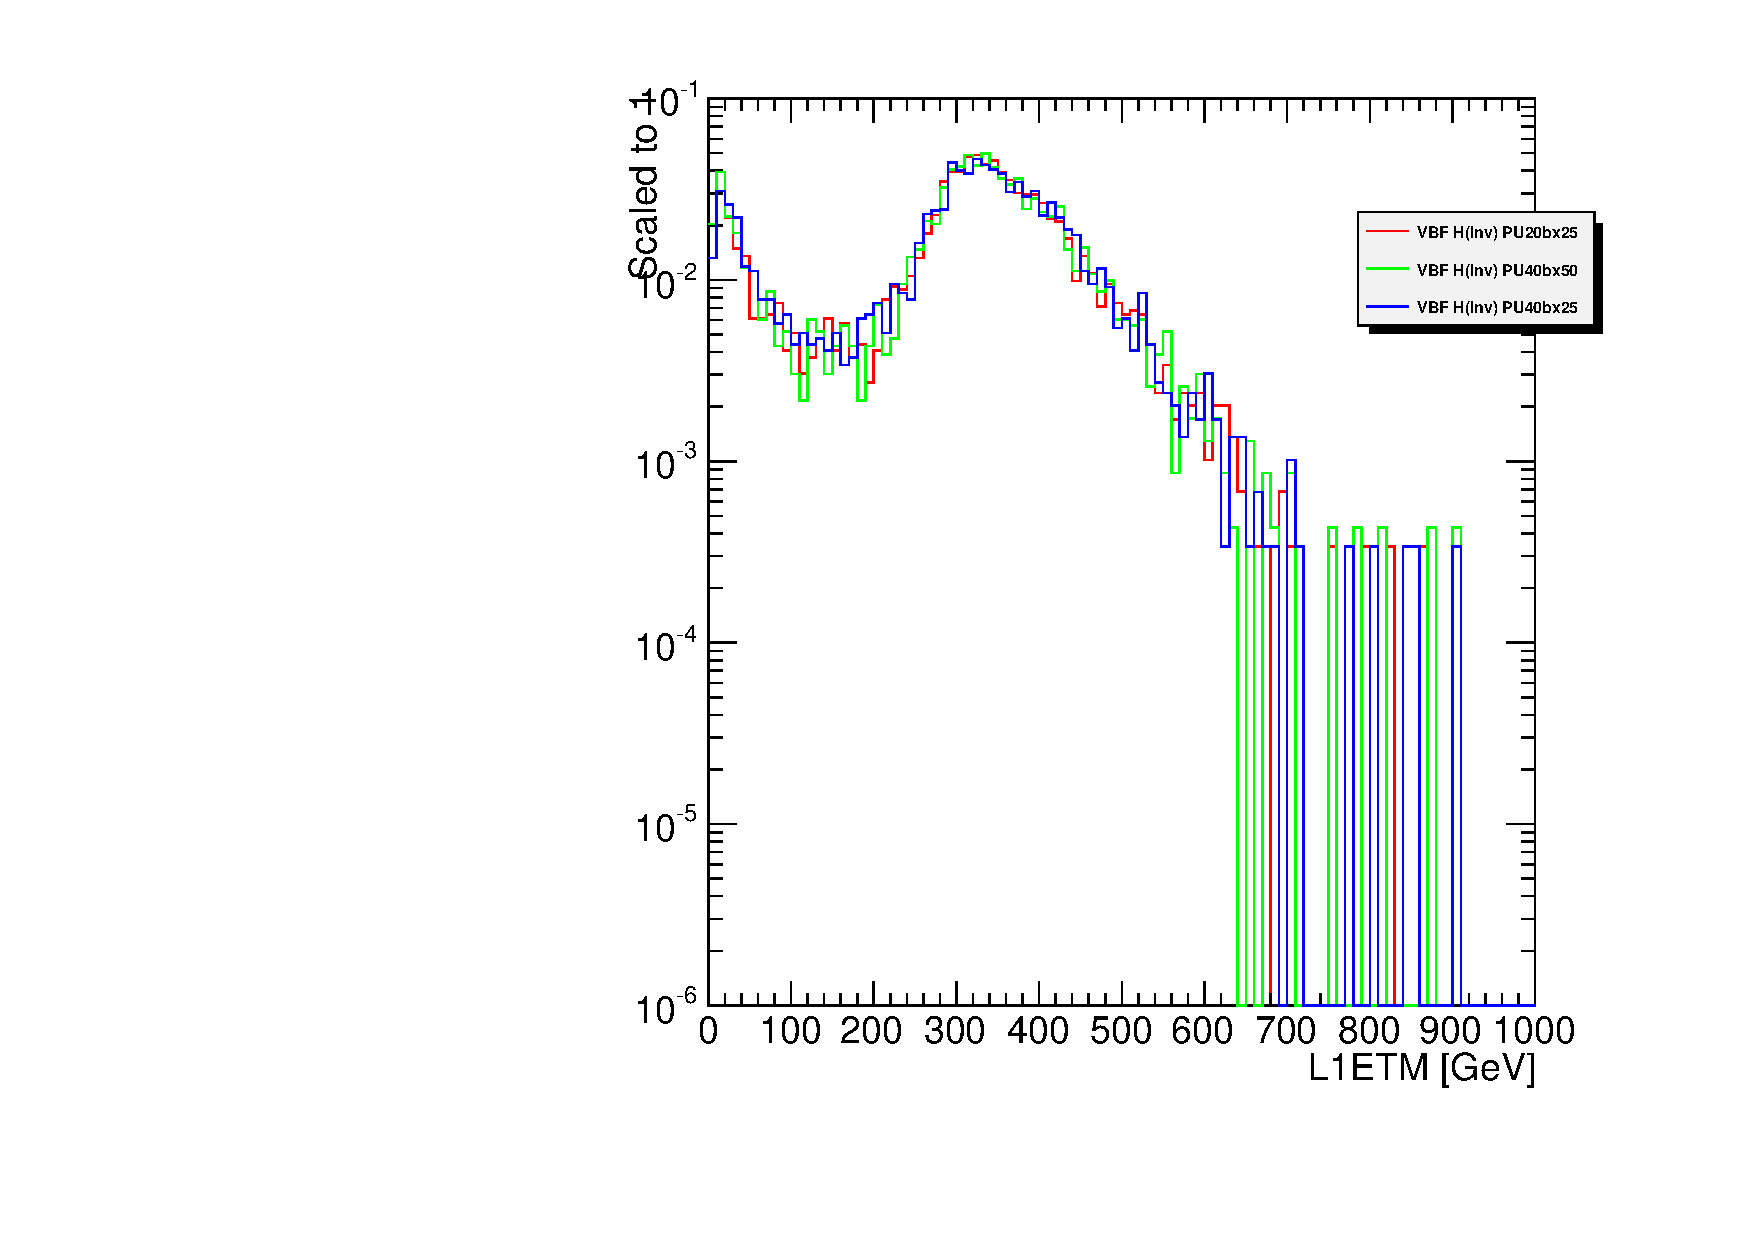
\includegraphics[width=\linewidth]{fig/L1ETM_Saturated_Sig.pdf}

\end{block}

\end{columns}

As expected events with at least on part of the calorimeter system saturated show higher L1\_ETM.

\end{frame}

% ###################################################
\begin{frame}{Loking at ETM on saturated events II}

\begin{columns}
 
\column[t]{0.45\linewidth}
\begin{block}{VBF H(Inv) event populations}
\centering

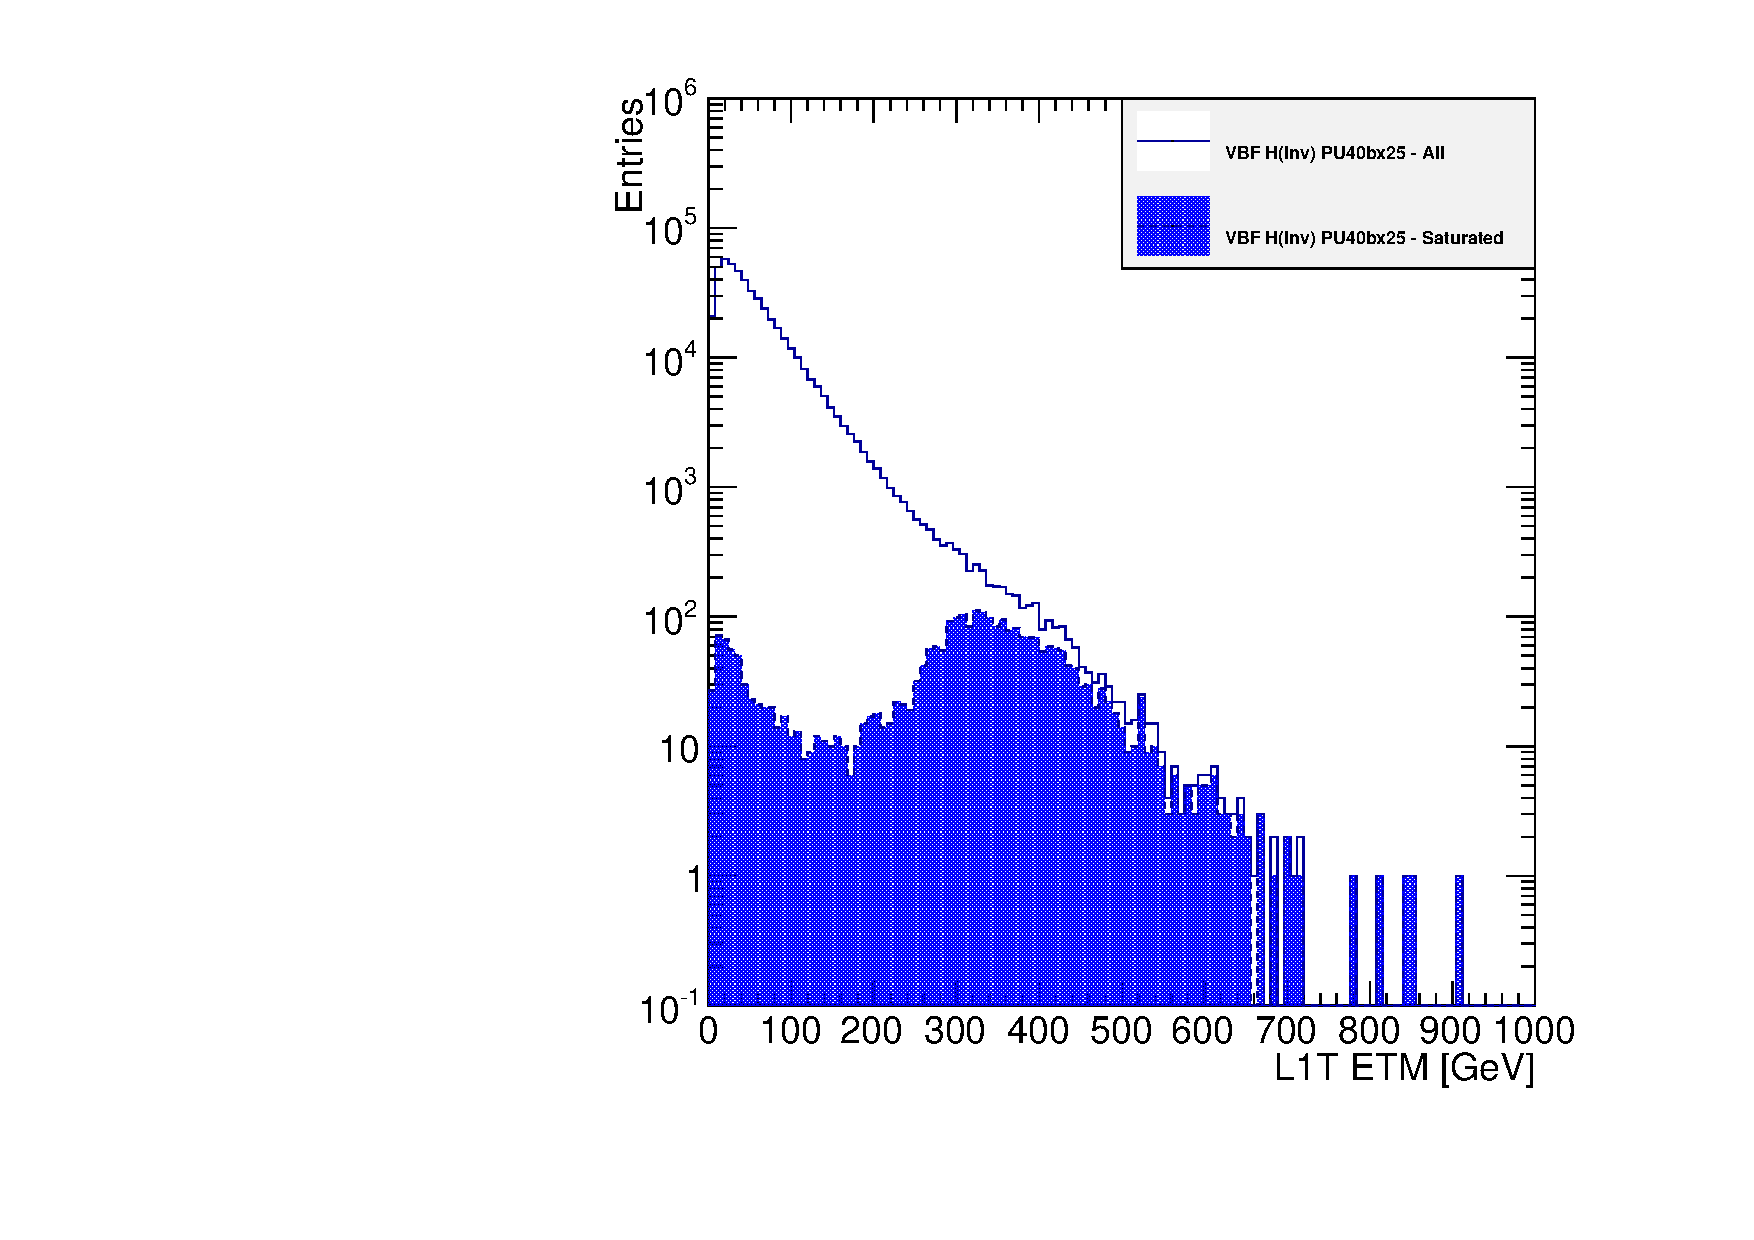
\includegraphics[width=\linewidth]{fig/L1ETM_Overlap.pdf}

\end{block}

\column[t]{0.45\linewidth}
\begin{block}{Notes}

\begin{itemize}
  \item We can see that at about L1\_ETM300 about \%50 of the events are saturated 
  \item We can see that at about L1\_ETM400 almost all events are saturated
  \item This is not a problem now but can be with increasing PU. More saturated events will happen.
\end{itemize}

\end{block}

\end{columns}
 
\end{frame}

% ###################################################
\begin{frame}{Loking at HTT on saturated events}

Now we can have a look at the properties of events of saturated ECAL TT (value=255), HCAL TT (value=255) or RCT Regions (value=511):

\begin{columns}
 
\column[t]{0.45\linewidth}
\begin{block}{All events}
\centering

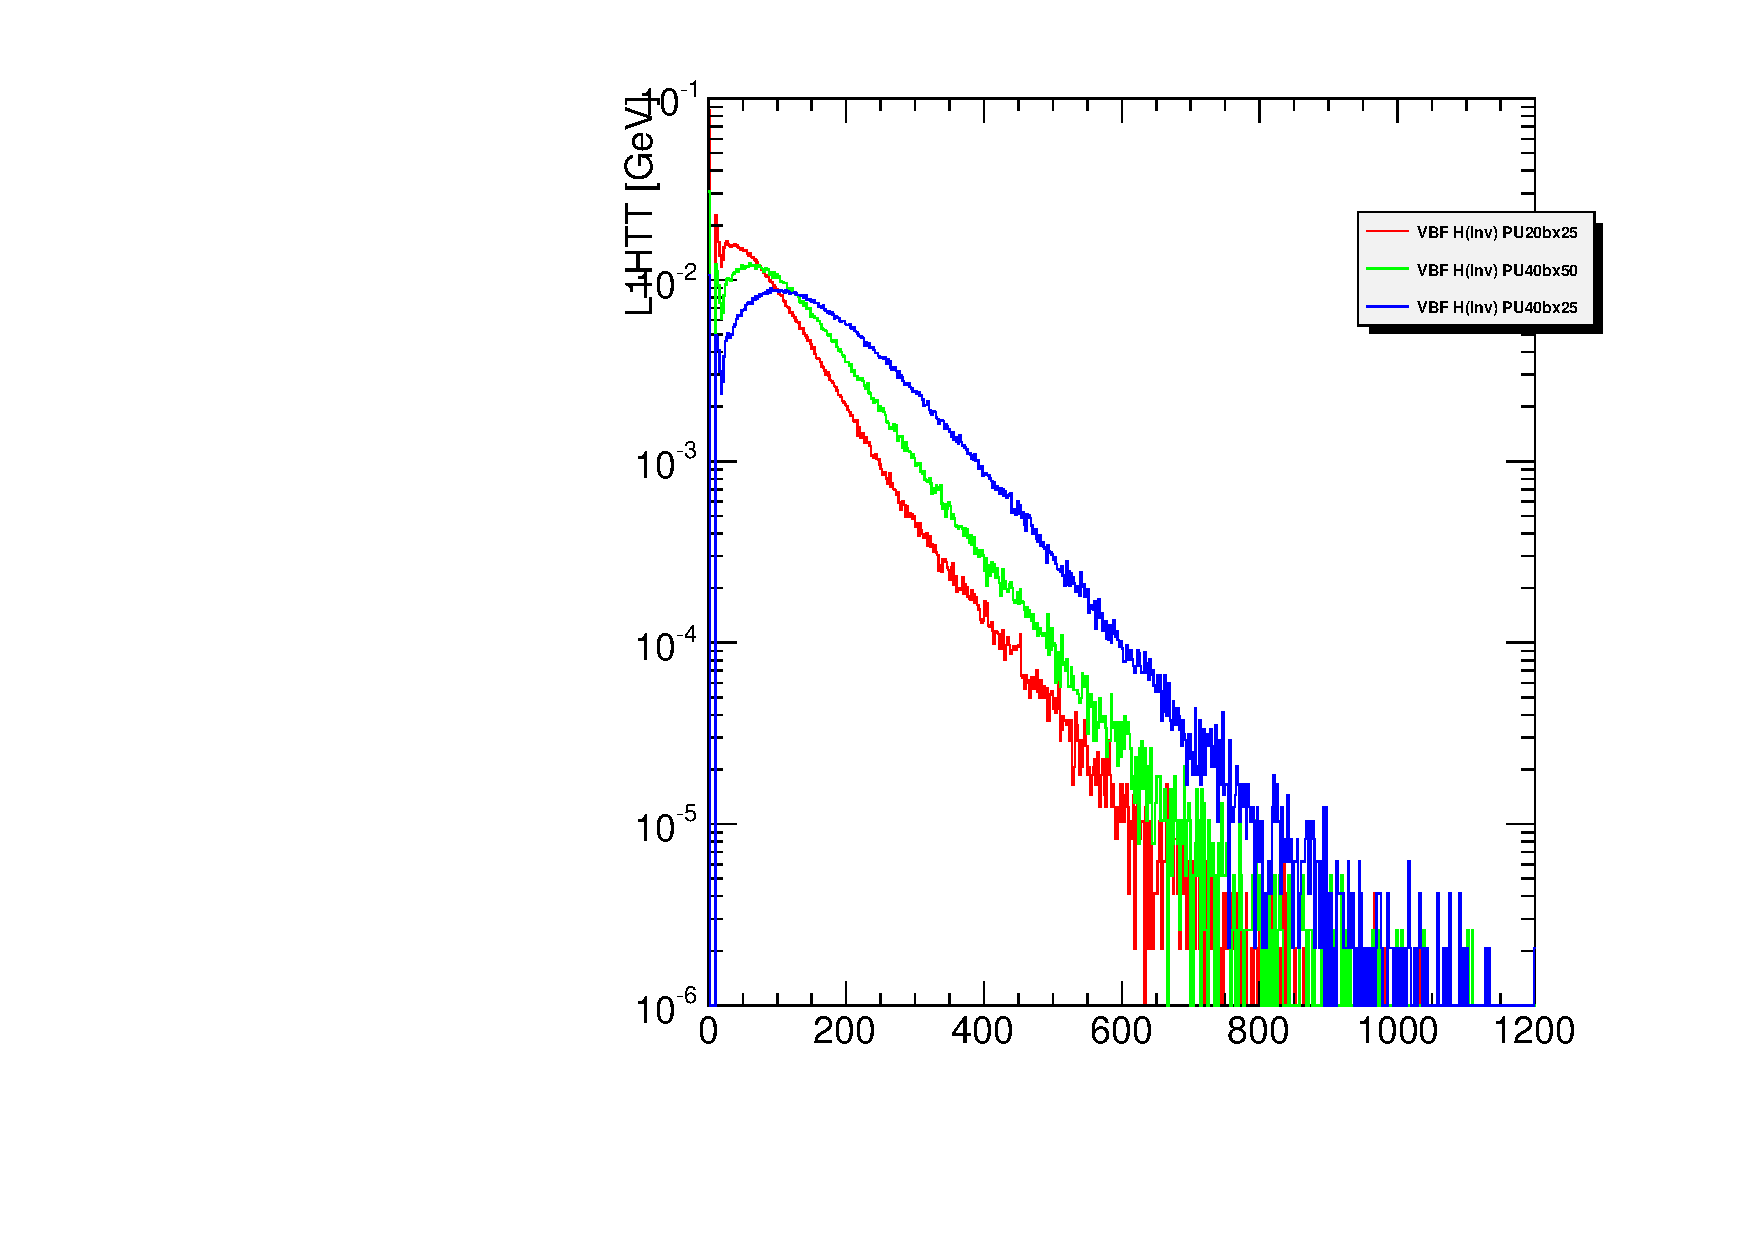
\includegraphics[width=\linewidth]{fig/L1HTT_Sig.pdf}

\end{block}

\column[t]{0.45\linewidth}
\begin{block}{VBF H(Inv)}
\centering

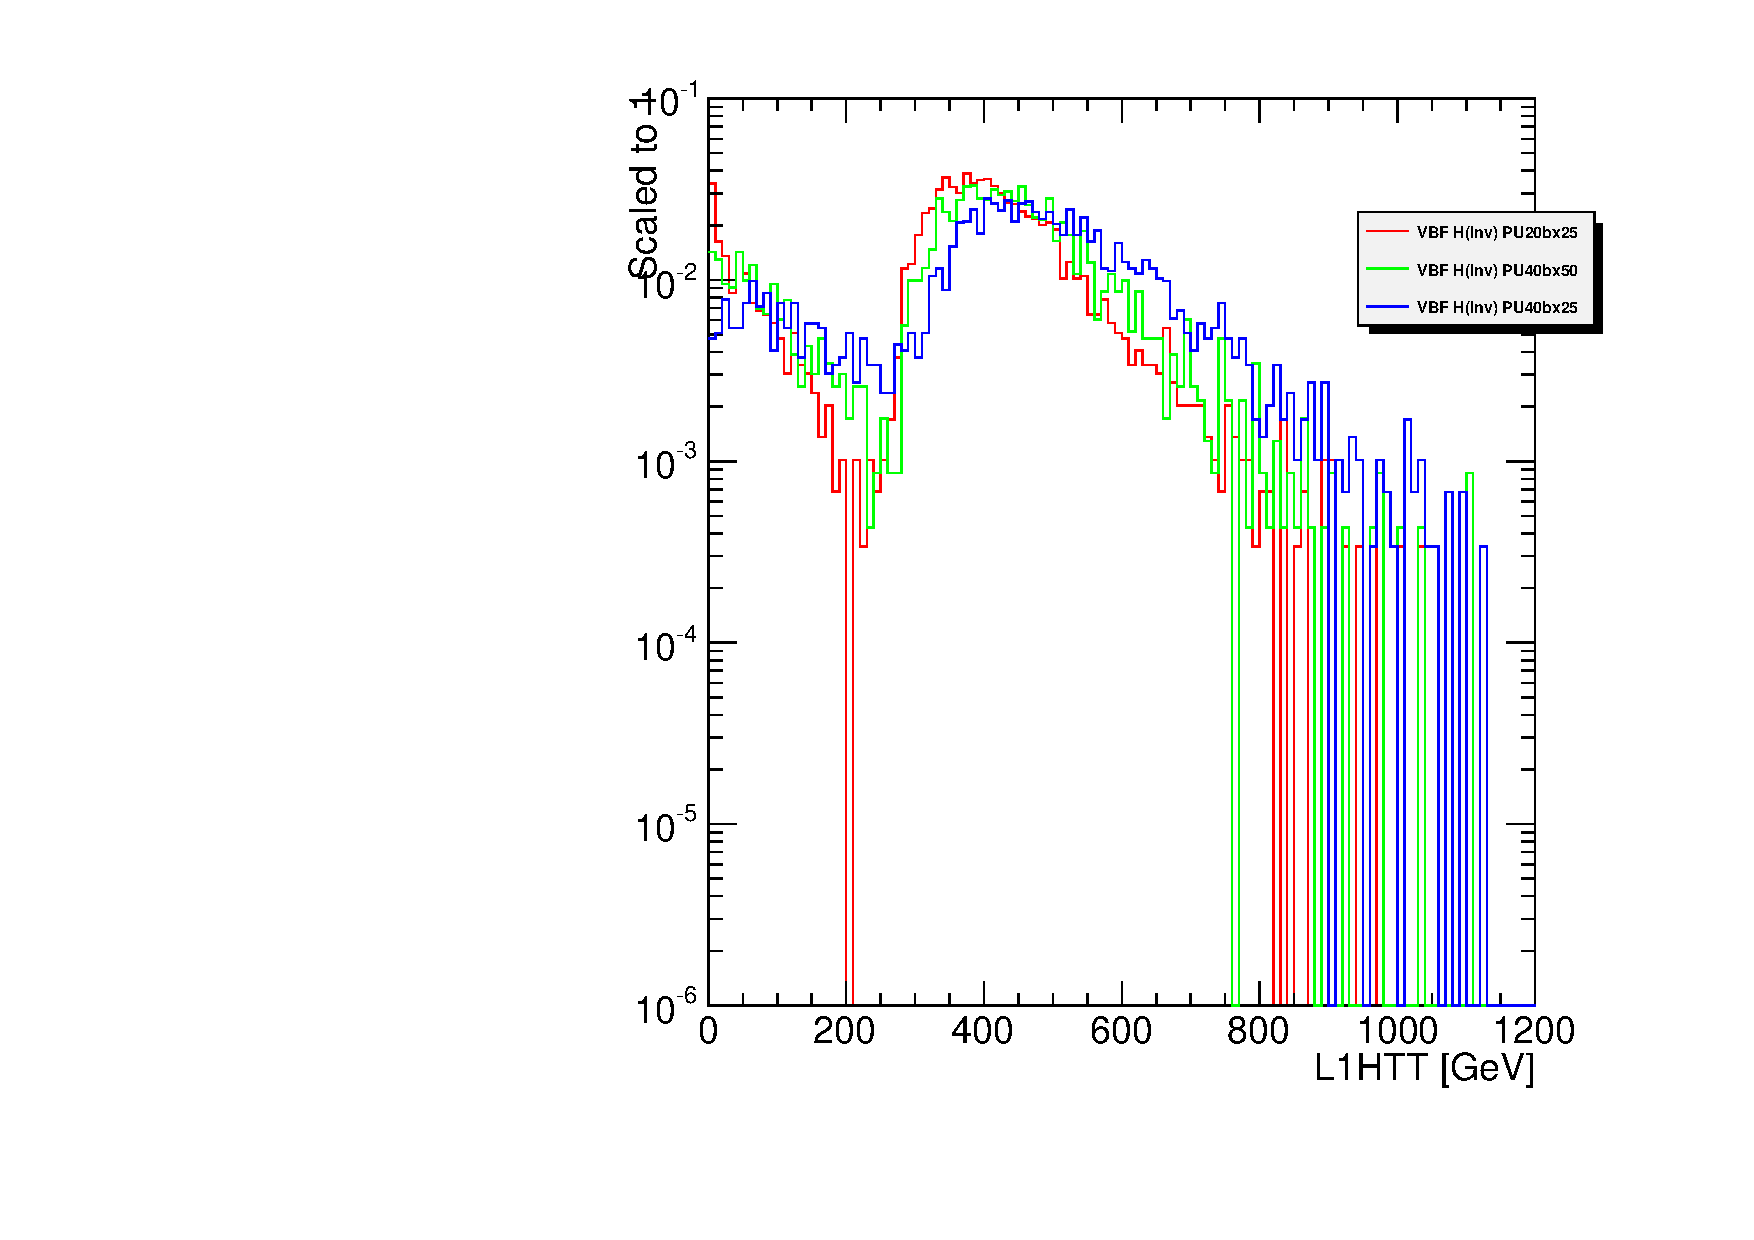
\includegraphics[width=\linewidth]{fig/L1HTT_Saturated_Sig.pdf}

\end{block}

\end{columns}

In the case of HTT events of saturated calorimeter parts are more rare and do not influence the shape so much. Also (for now) we are not considering this variable for seed.

\end{frame}

\section{ECAT TT 127 peak investigation}

% ###################################################
\begin{frame}{TT Mapping}

\begin{columns}
 
\column[t]{0.45\linewidth}
\begin{block}{TT and RCT regions map}
\centering

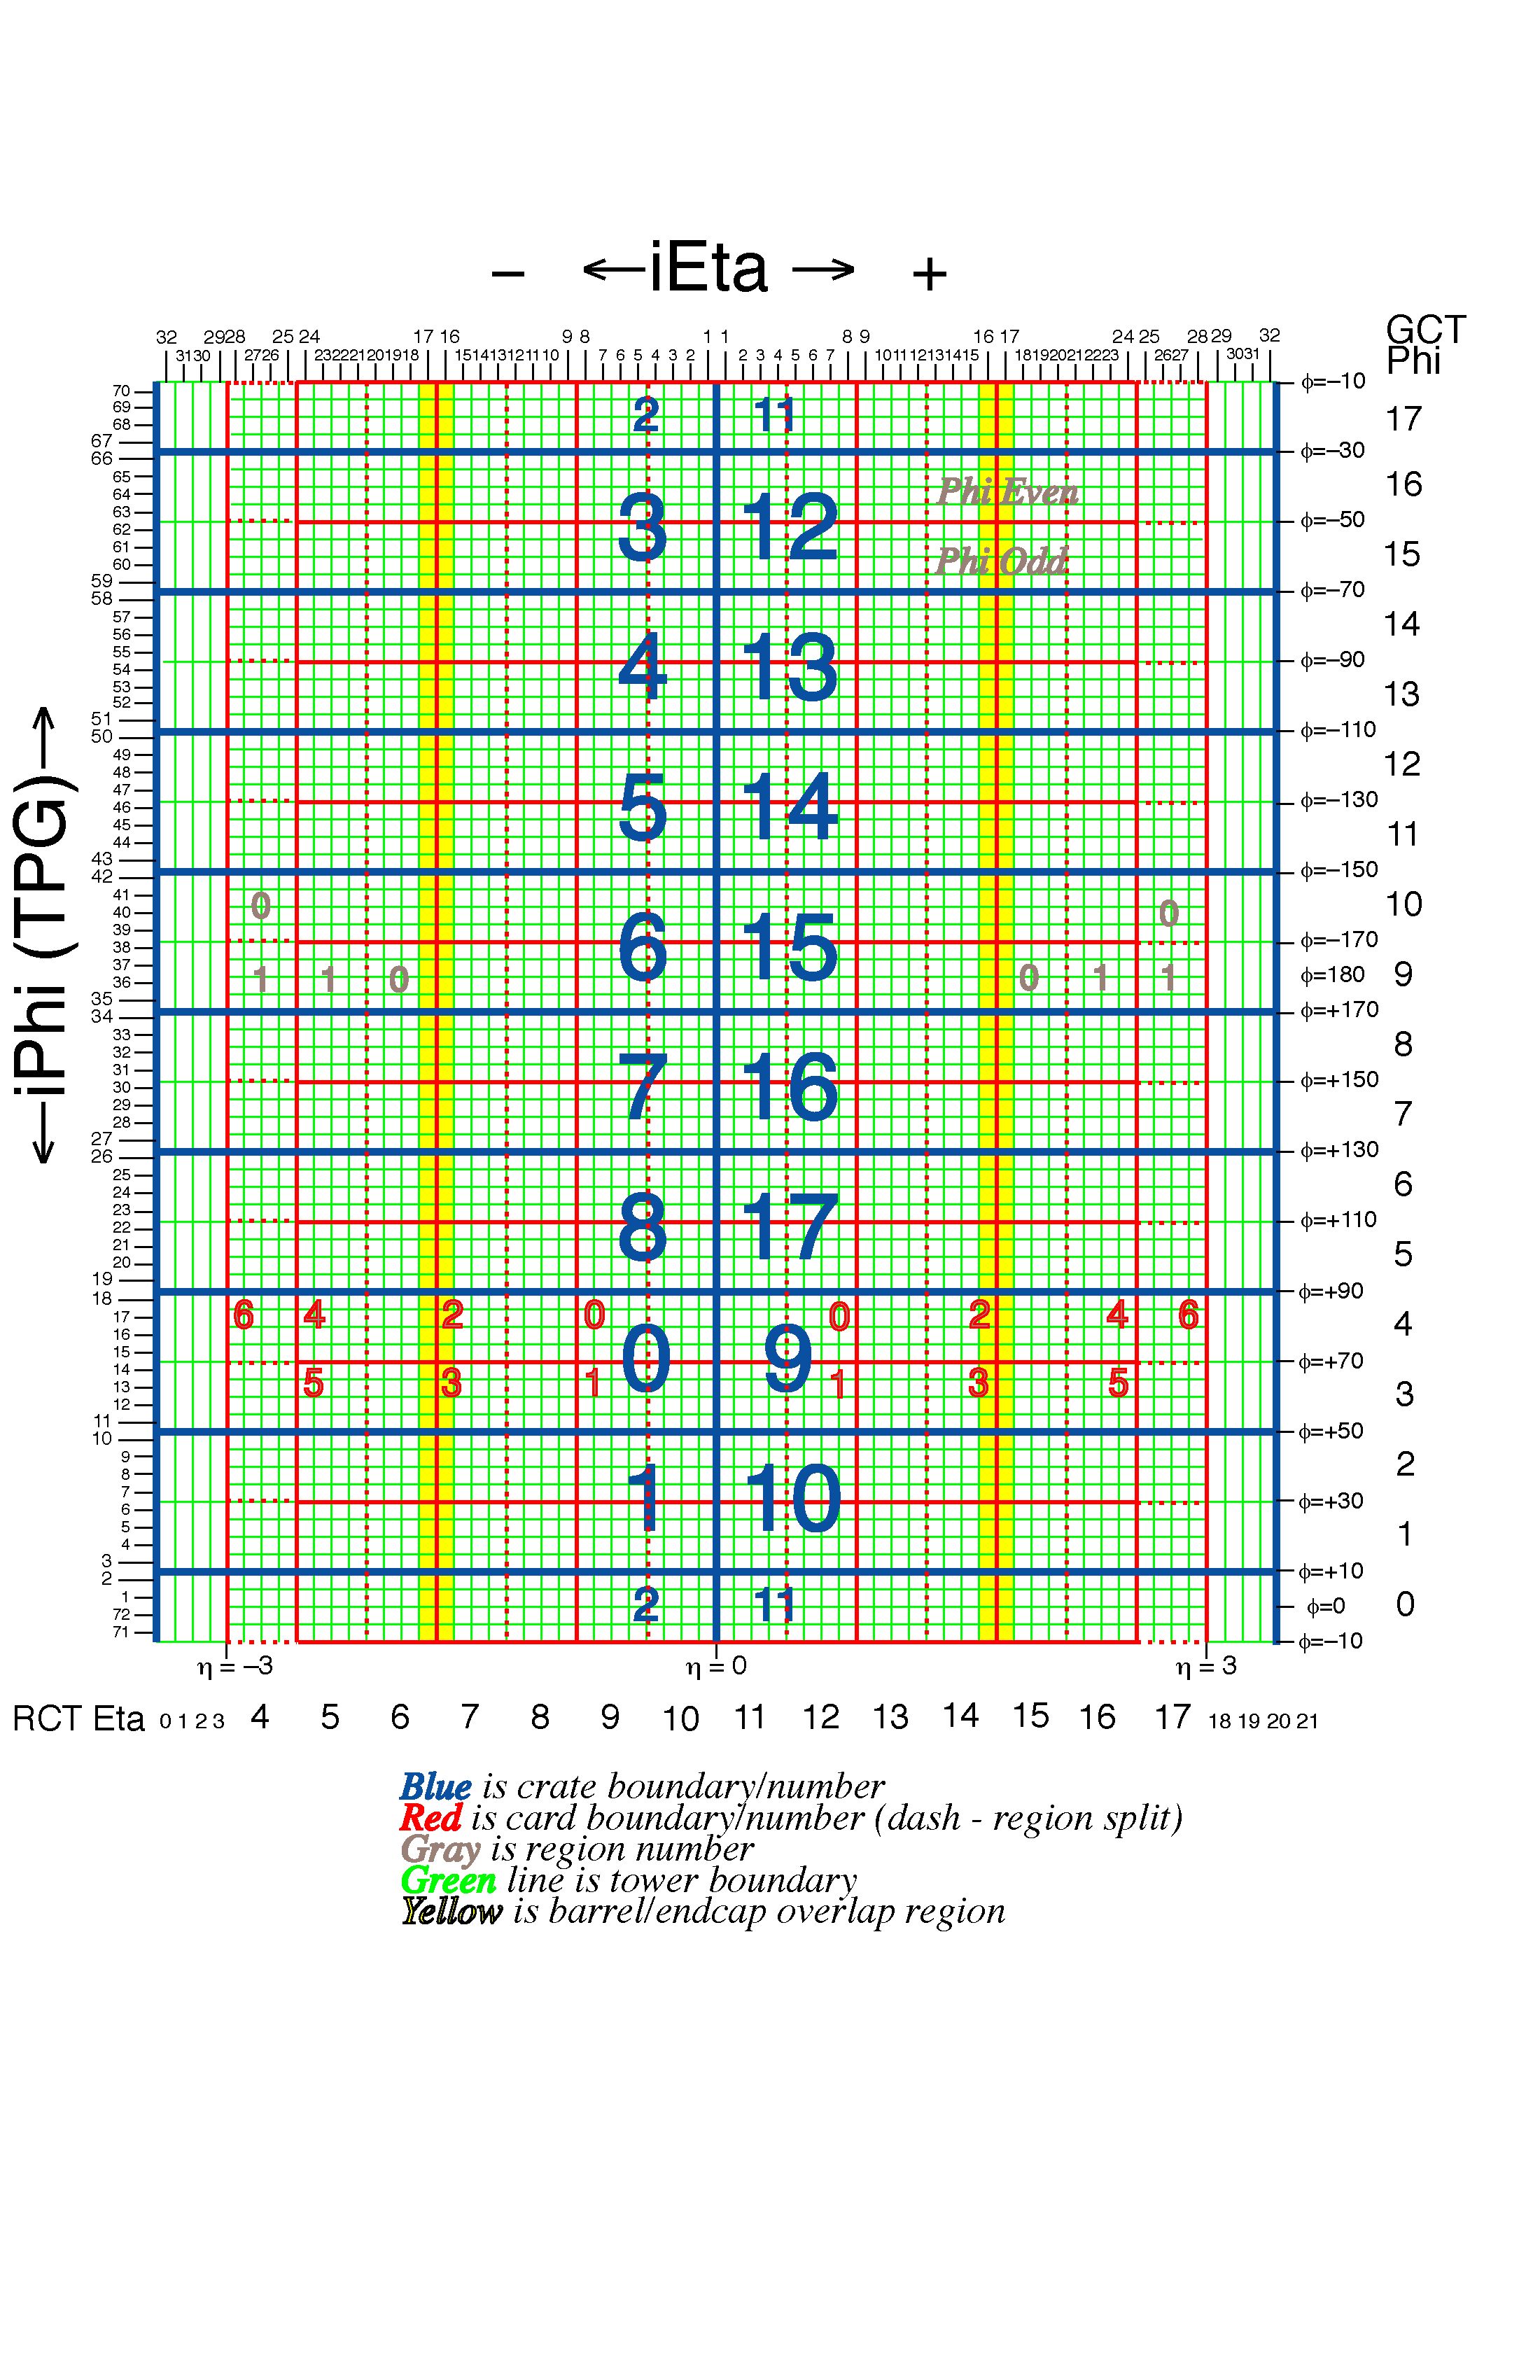
\includegraphics[width=0.8\linewidth]{fig/towers_ieta_iphi_2009.png}

\end{block}

\column[t]{0.45\linewidth}
\begin{block}{Notes}
\centering

\begin{itemize}
 \item For future reference this is the map of the RCT regions and ECAL/HCAL TT.
 \item This allows for conversion from ieta and iphi units and eta and phi.
 \item We can see that the barrel/encap overlap region is at $|ieta|=16,17$
 \item We can see that ECAL ends at $eta=3.0$ which is $|ieta|=28$
\end{itemize}

\end{block}

\end{columns}

\end{frame}

% ###################################################
\begin{frame}{Investigating ECAL TT peak at 127}

First suggestion was to look at ECAL TT at between barrel and endcaps

\begin{columns}
 
\column[t]{0.45\linewidth}
\begin{block}{Barrel (TT $ieta<17$)}
\centering

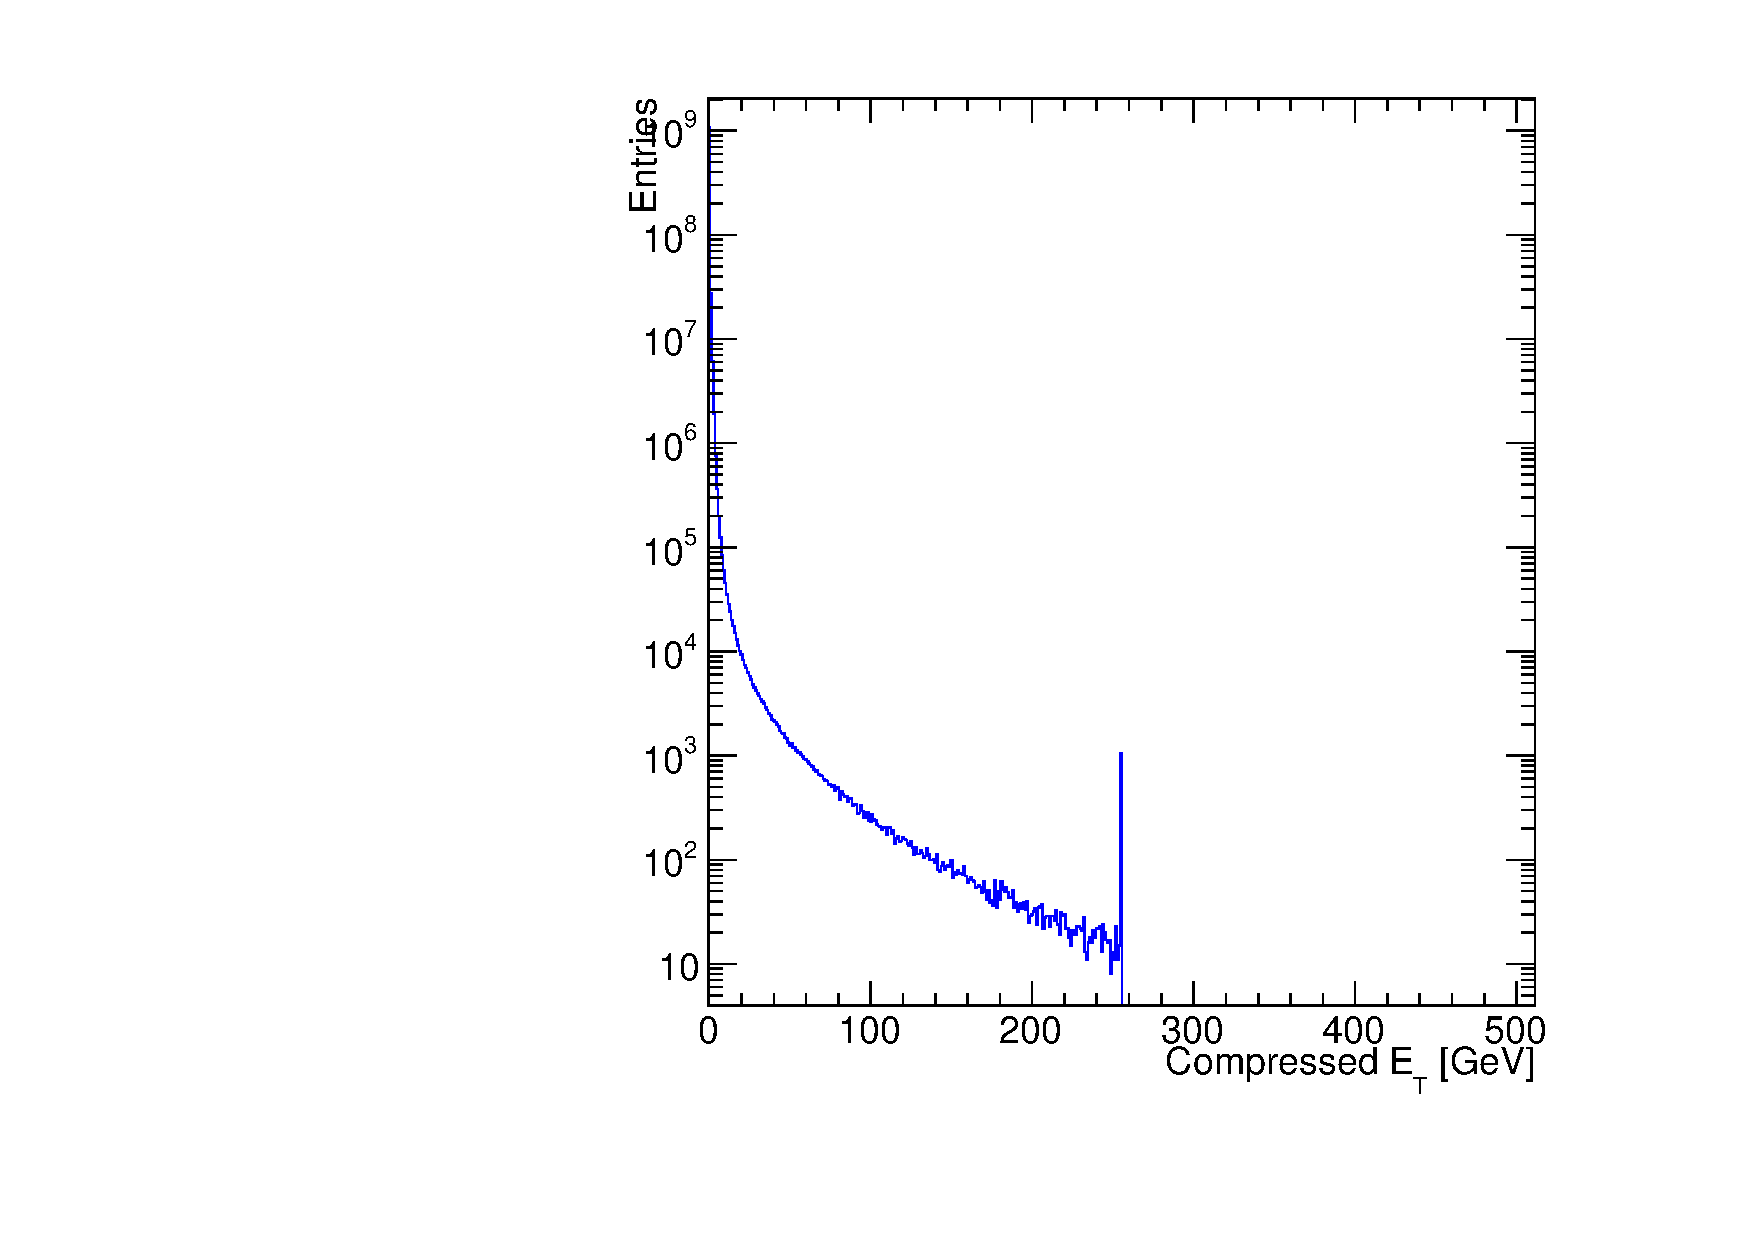
\includegraphics[width=\linewidth]{fig/ECALTT_Barrel_CompressedEt.pdf}

\end{block}

\column[t]{0.45\linewidth}
\begin{block}{Endcap (TT $ieta>=17$)}
\centering

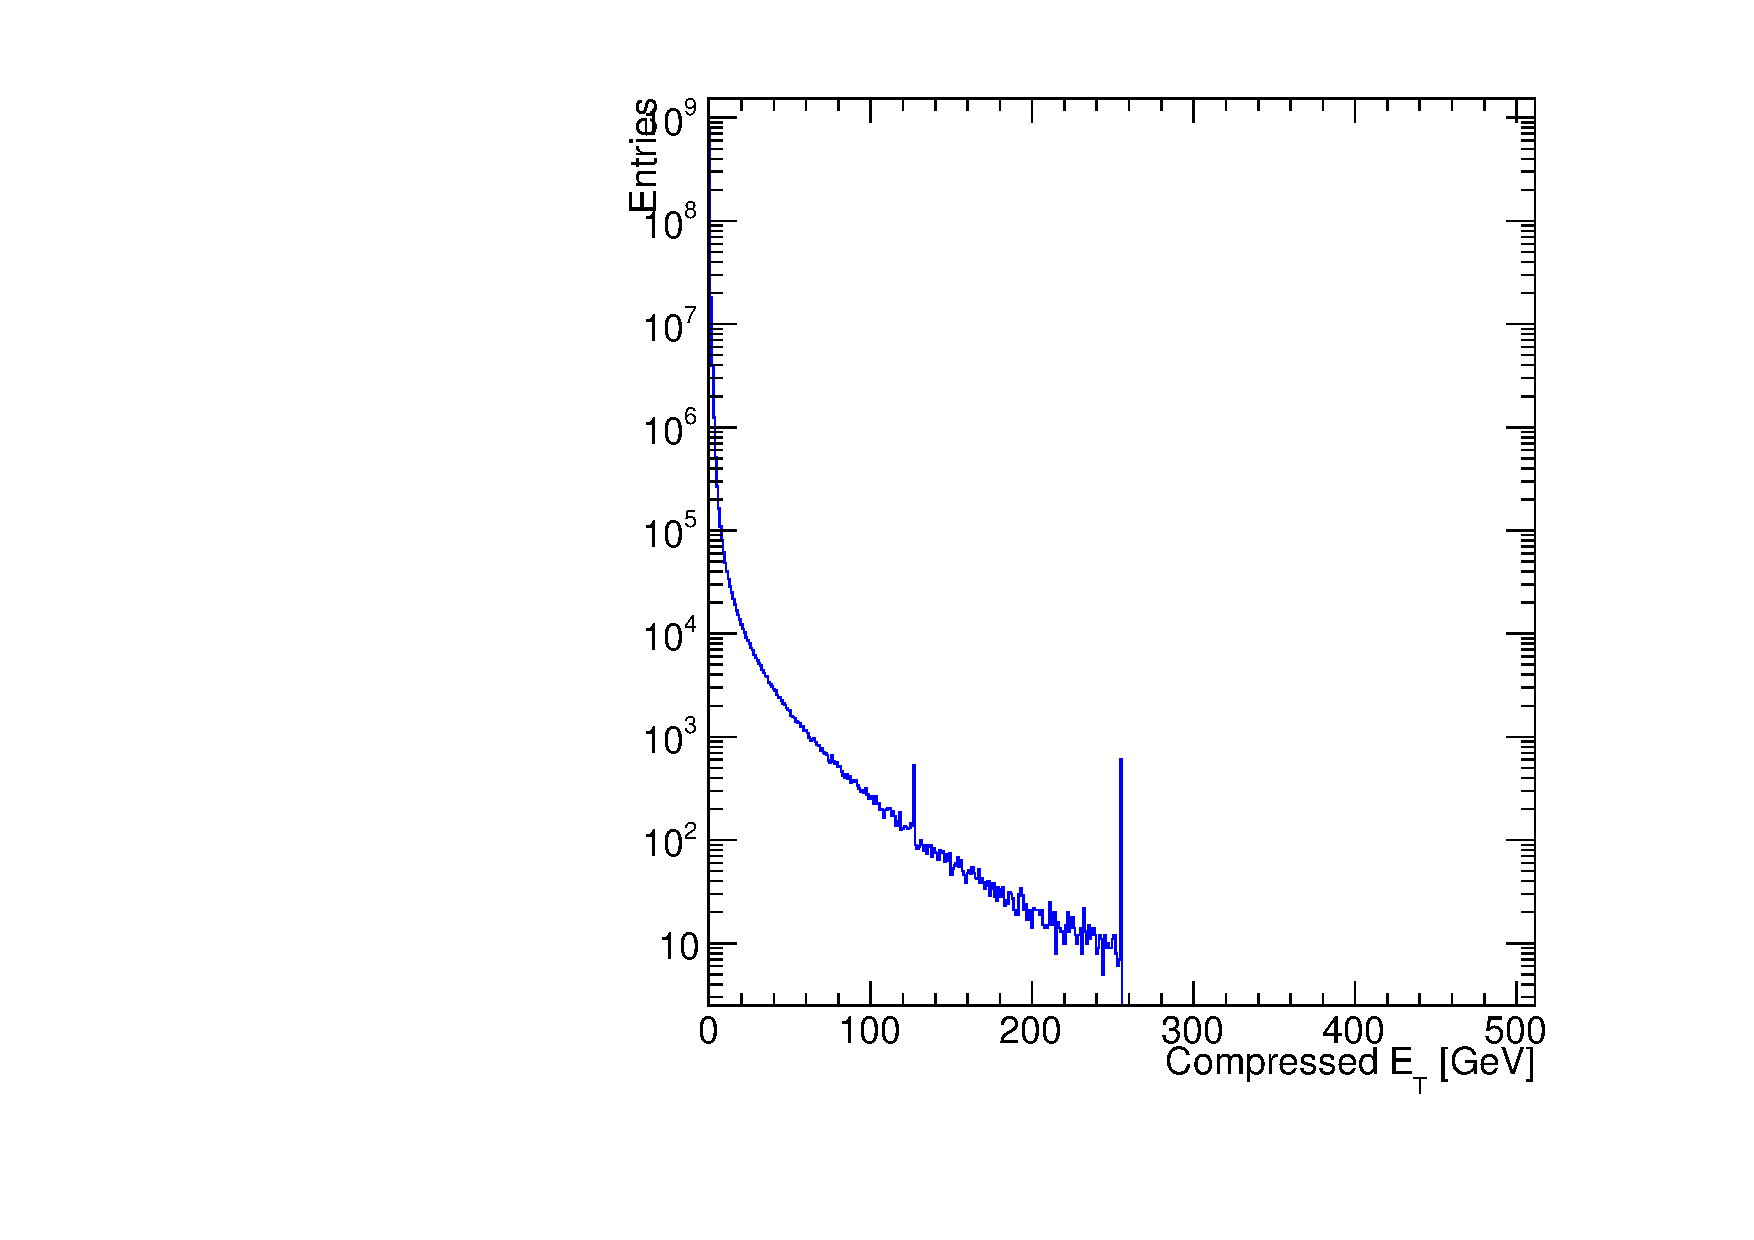
\includegraphics[width=\linewidth]{fig/ECALTT_Endcap_CompressedEt.pdf}

\end{block}

\end{columns}

We can see that the effect is confined to endcaps!

\end{frame}

% ###################################################
\begin{frame}{Investigating ECAL TT peak at 127}

Mapping of all events that have ECAL TT equal to 127

\begin{columns}
  
\column[t]{0.45\linewidth}
\begin{block}{Distribution of TT}
\centering

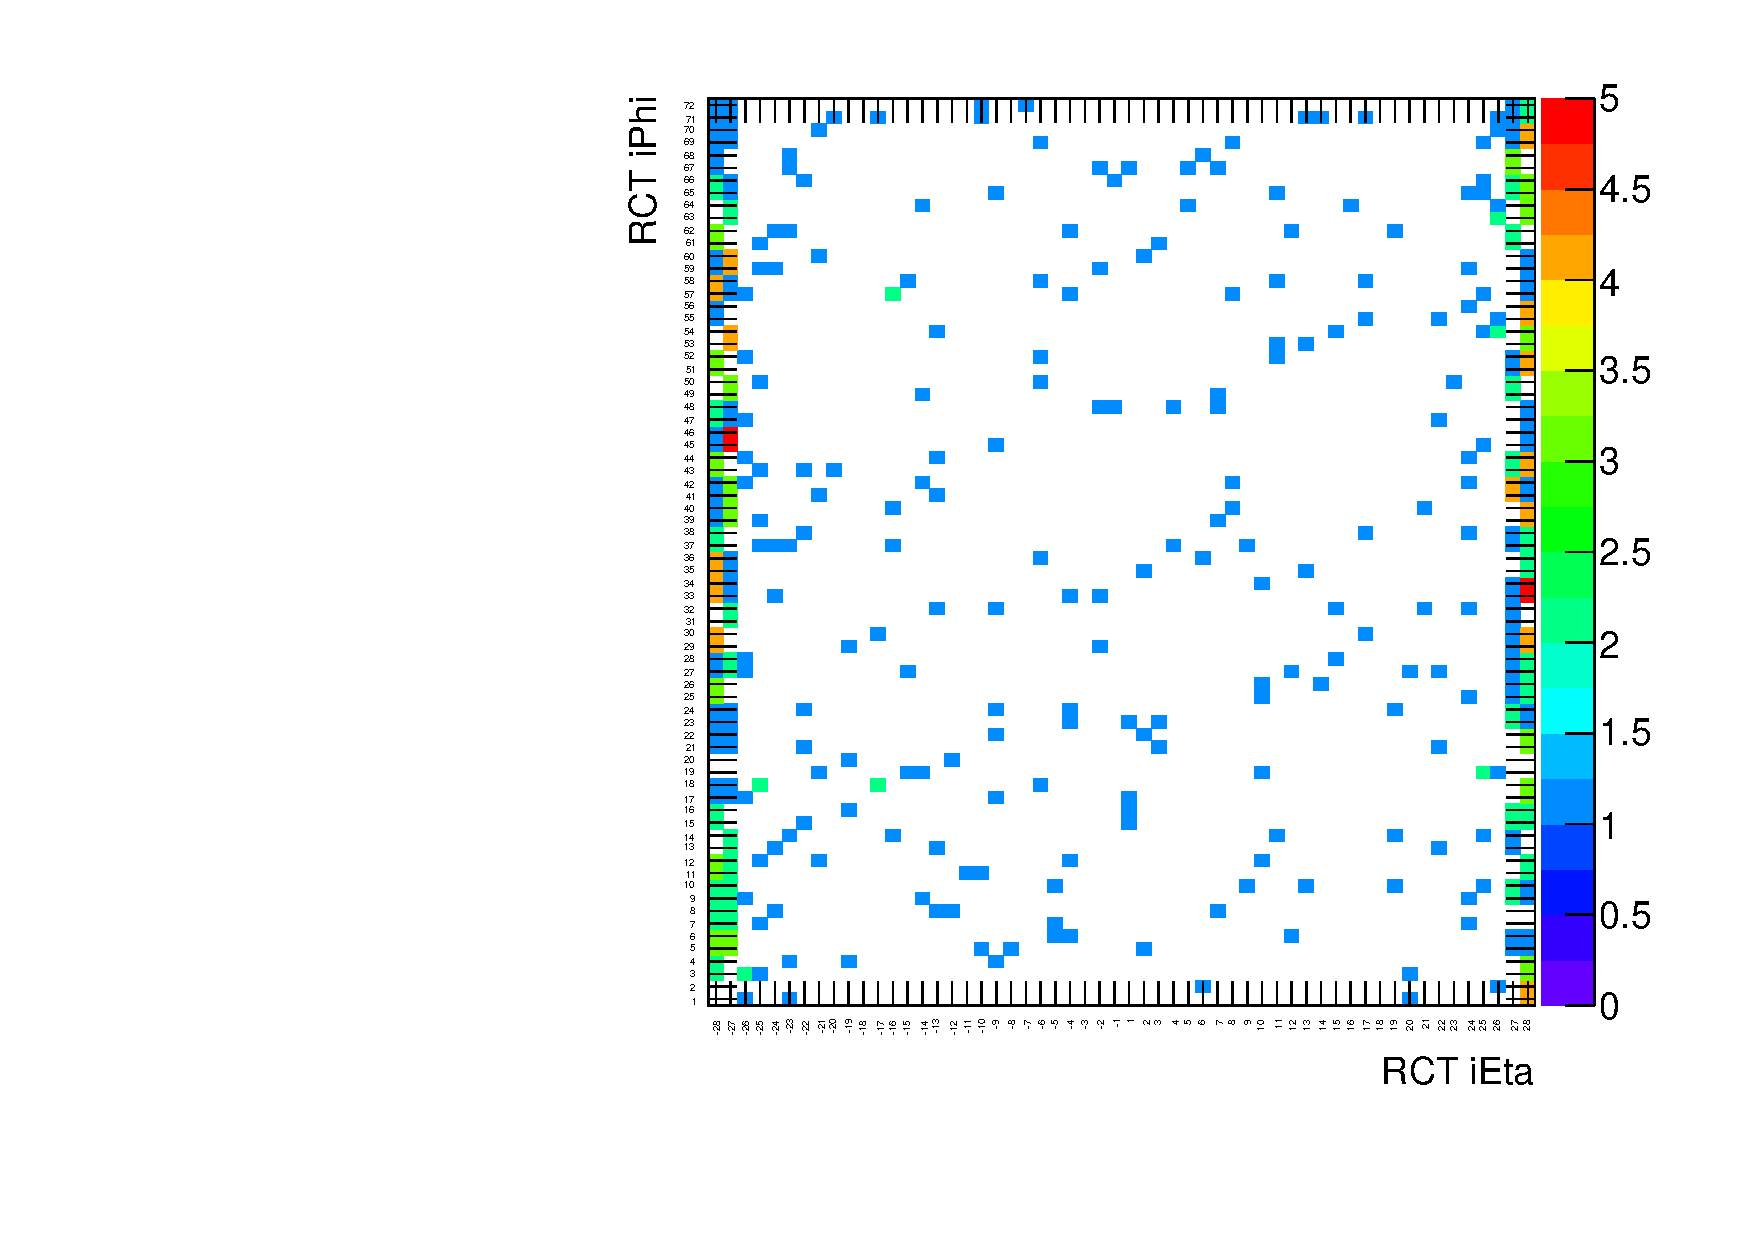
\includegraphics[width=\linewidth]{fig/ECALTT_CompressedEt127_EtaPhiTotal.pdf}

\end{block}

\column[t]{0.45\linewidth}
\begin{block}
\centering

We can see that a large concentration of event at the end of the endcaps $ieta=27,28$
\begin{itemize}
  \item Is there anything special about this ECAL TT? I know they have strange geometries and less then 25 crystals... but should also have 8 bits coming out no?
  \item This can be a real effect (also present on data) or just a simulation effect (just on MC)
  \item If this is a real saturation (no more that 127 is possible in those towers) this will be easier to saturate specially by VBF like jets, making basically VBF+jets signature at L1... this may be a problem.
\end{itemize}

\end{block}

\end{columns}



\end{frame}

% ###################################################
\begin{frame}{Summary and next steps}
 
\begin{block}{Summary:}
 
\begin{itemize}
  \item First look at L1\_ETM\_X + HLT path to calculate signal efficiency if we do nothing and signal loss is $\sim25-30\%$
  \item Different trends in parked triggers are now understood.
  \item Saturation will not be a problem for rates (neutrino gun studies) but will change a small fraction of our signal shapes at L1 (more L1\_ETM40 better? even if from saturation?).
  \item Investigation of ECAL TT 127 peak study underway, apparently found a "maybe unknown" problem in the detector or simulation. 
\end{itemize}

\end{block}

\begin{block}{Next Steps:}
 
\begin{itemize}
  \item Calculate VBF signal efficiency assuming SUSY L1 proposals (some are very interesting using MHT/HTT which should work for us).
  \item Re-calculate everything for UCT L1 objects.
  \item Investigate the ECAL TT 127 peak and pass information to the relevant group.
\end{itemize}
 
\end{block}

\end{frame}

% ###################################################
\appendix
% ###################################################
\begin{frame}
 
\begin{block}

\begin{center}Backup Slides\end{center}

\end{block}

\end{frame}

% {
% \setbeamercolor{background canvas}{bg=}
% \includepdf[pages=11]{hinv\_magnan\_140506.pdf}
% }

% ###################################################
\begin{frame}{Parked HLT seed composition I}

\begin{columns}
 
\column[t]{0.45\linewidth}
\begin{block}{\footnotesize HLT\_DiJet20\_MJJ650\_AllJets\_DEta3p5\_HT120\_VBF\_v}
\centering

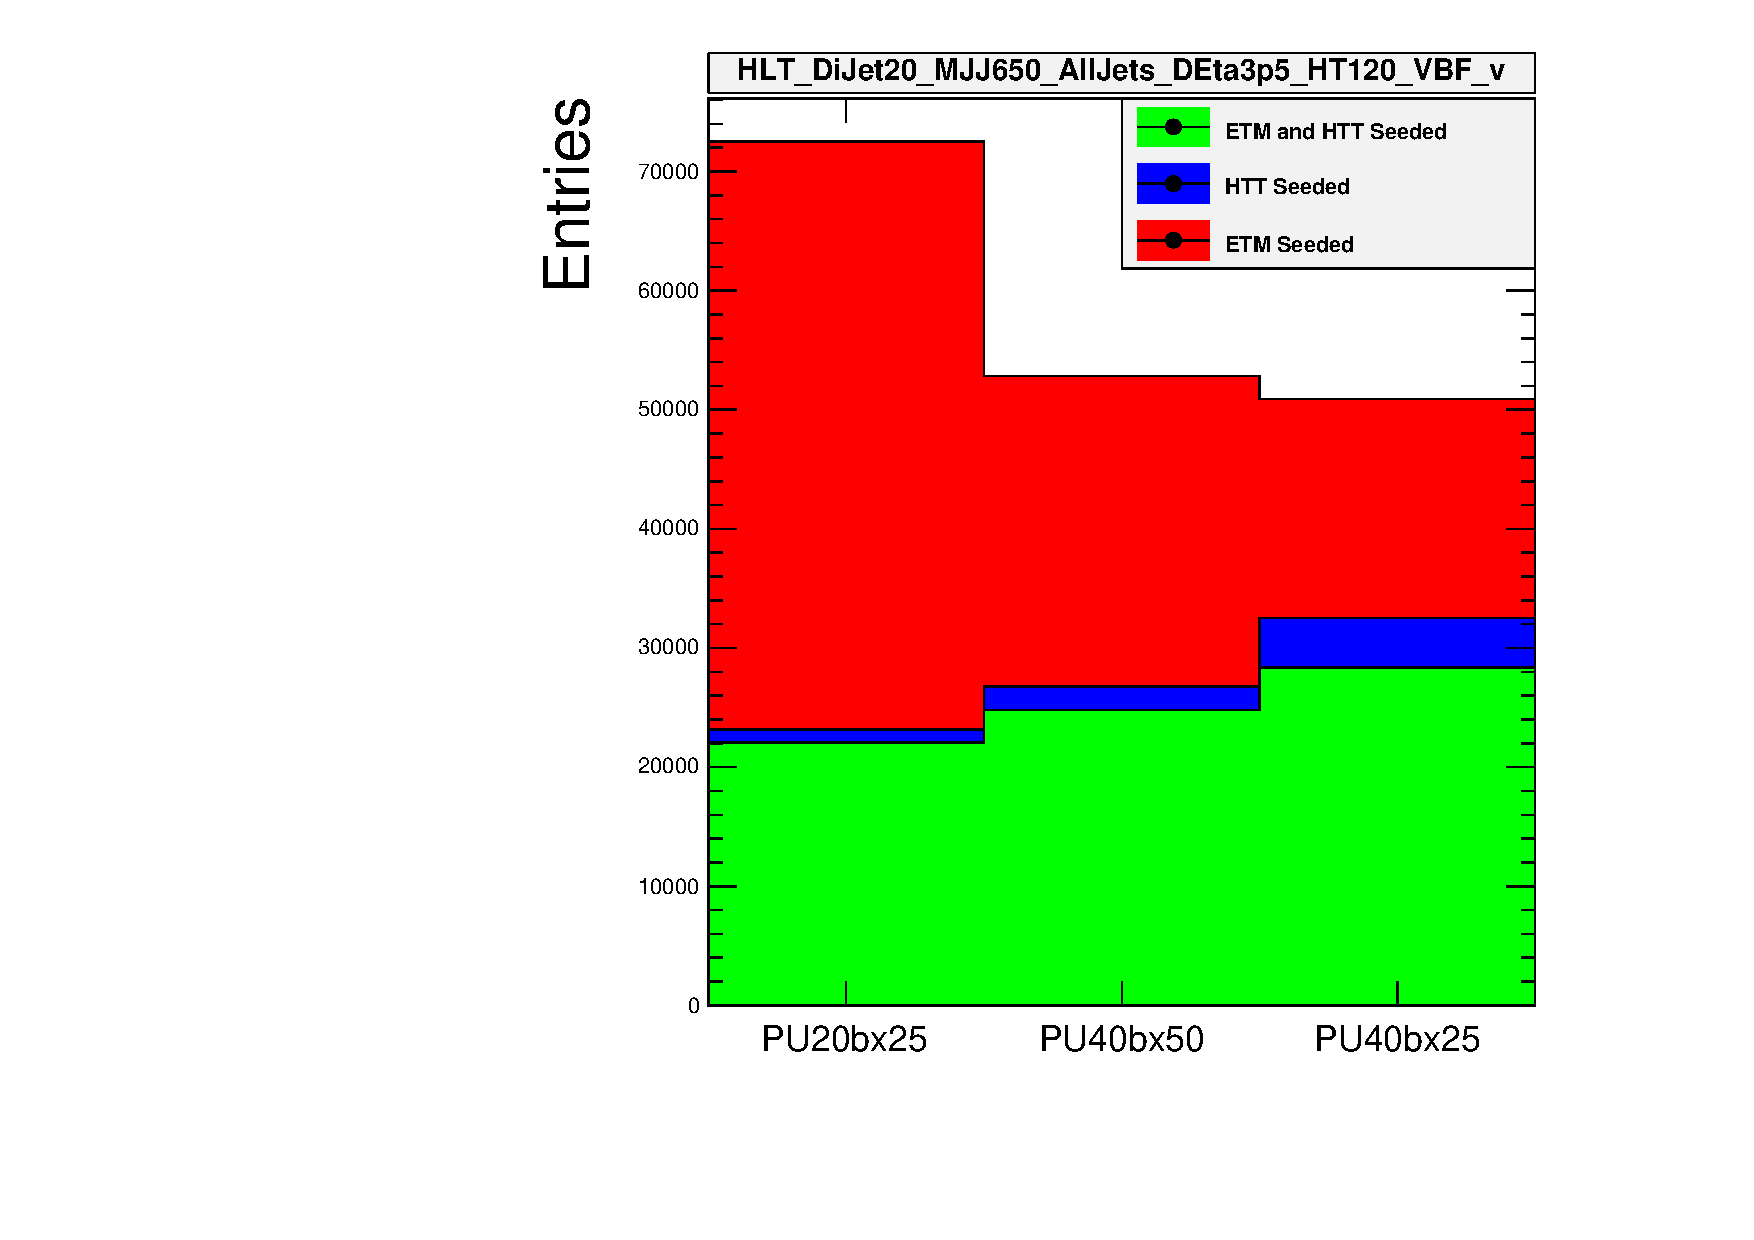
\includegraphics[width=\linewidth]{fig/HLT_DiJet20_MJJ650_AllJets_DEta3p5_HT120_VBF_v.pdf}

\end{block}
  
\column[t]{0.45\linewidth}
\begin{block}{\footnotesize HLT\_DiJet30\_MJJ700\_AllJets\_DEta3p5\_VBF\_v}
\centering

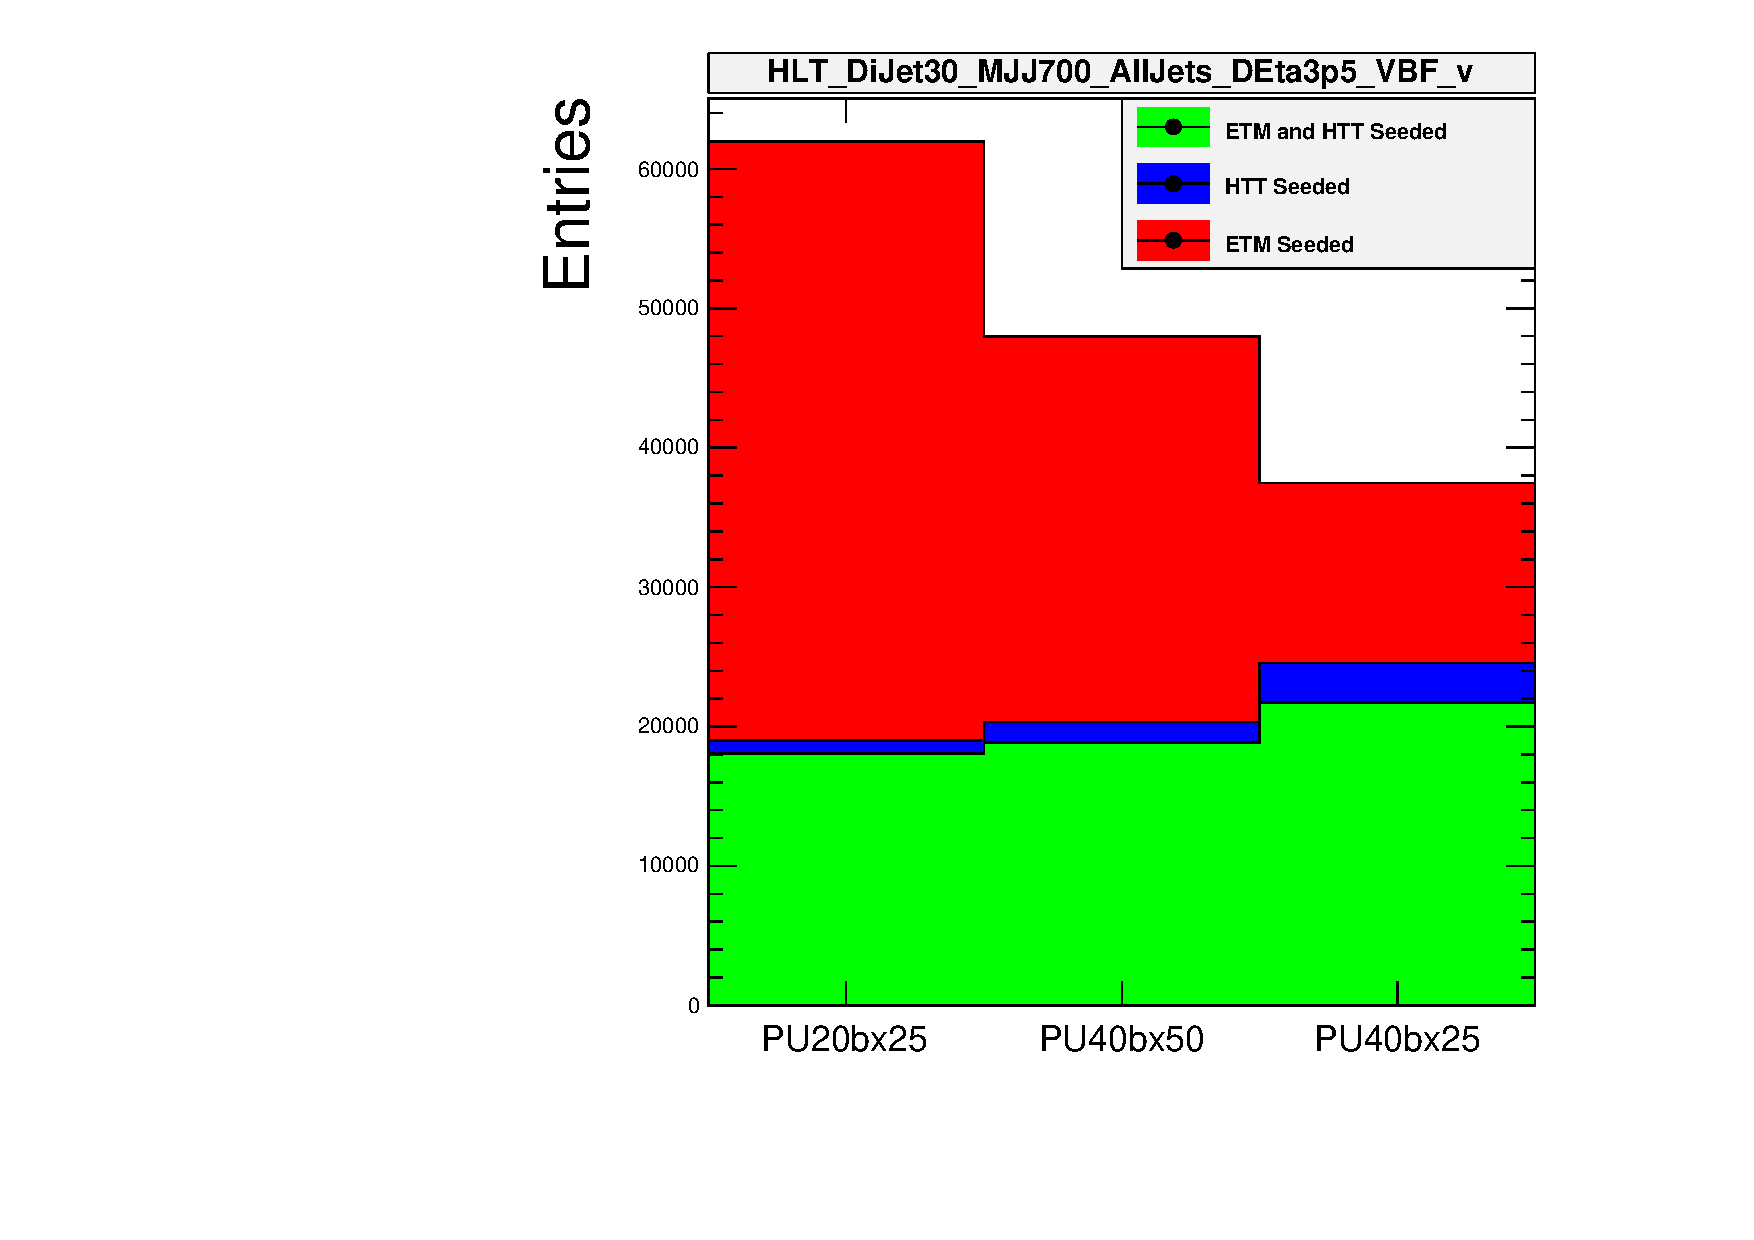
\includegraphics[width=\linewidth]{fig/HLT_DiJet30_MJJ700_AllJets_DEta3p5_VBF_v.pdf}

\end{block}

\end{columns}

\end{frame}

% ###################################################
\begin{frame}{Parked HLT seed composition II}

\begin{columns}
 
\column[t]{0.45\linewidth}
\begin{block}{\footnotesize HLT\_DiJet35\_MJJ650\_AllJets\_DEta3p5\_VBF\_v}
\centering

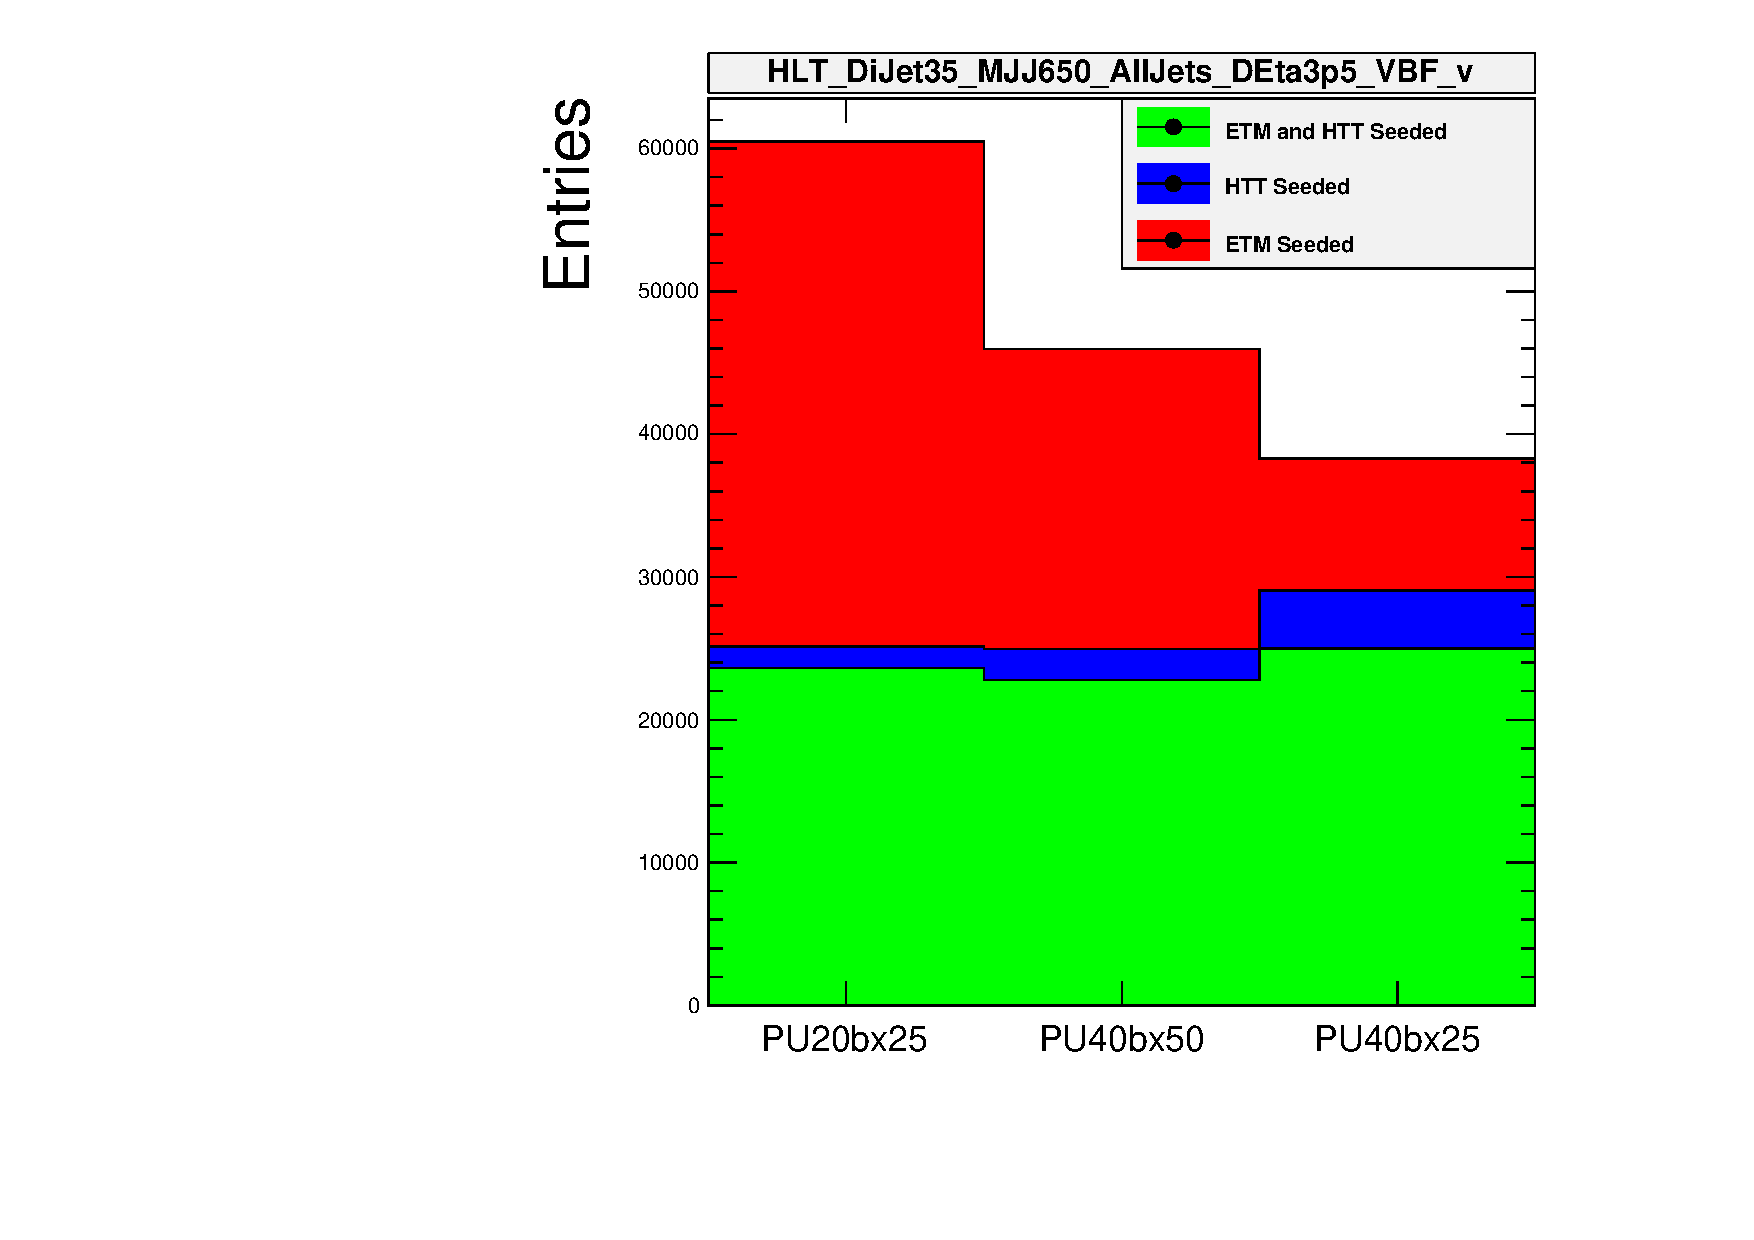
\includegraphics[width=\linewidth]{fig/HLT_DiJet35_MJJ650_AllJets_DEta3p5_VBF_v.pdf}

\end{block}
  
\column[t]{0.45\linewidth}
\begin{block}{\footnotesize HLT\_DiJet35\_MJJ700\_AllJets\_DEta3p5\_VBF\_v}
\centering

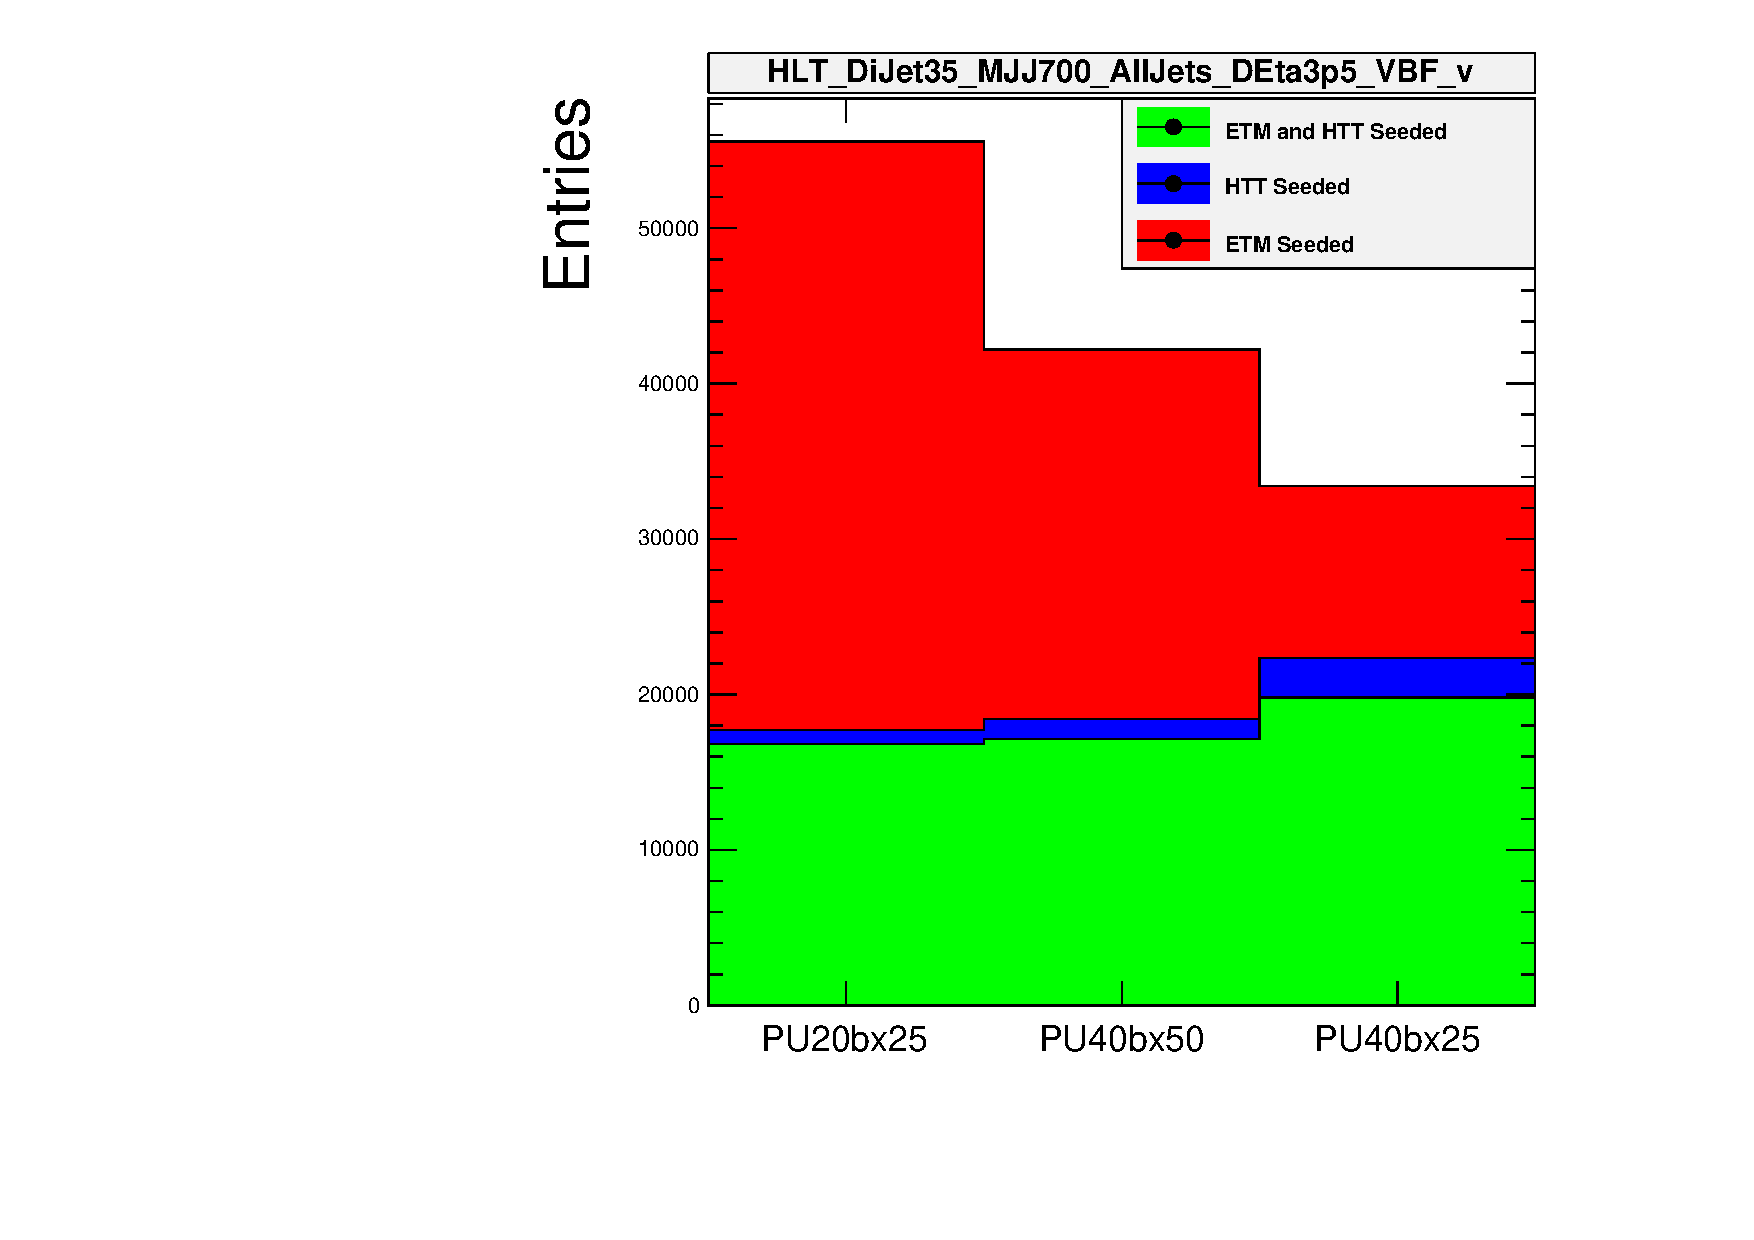
\includegraphics[width=\linewidth]{fig/HLT_DiJet35_MJJ700_AllJets_DEta3p5_VBF_v.pdf}

\end{block}

\end{columns}

\end{frame}

% ###################################################
\begin{frame}{Parked HLT seed composition III}

\begin{columns}
 
\column[t]{0.45\linewidth}
\begin{block}{\footnotesize HLT\_DiJet35\_MJJ750\_AllJets\_DEta3p5\_VBF\_v}
\centering

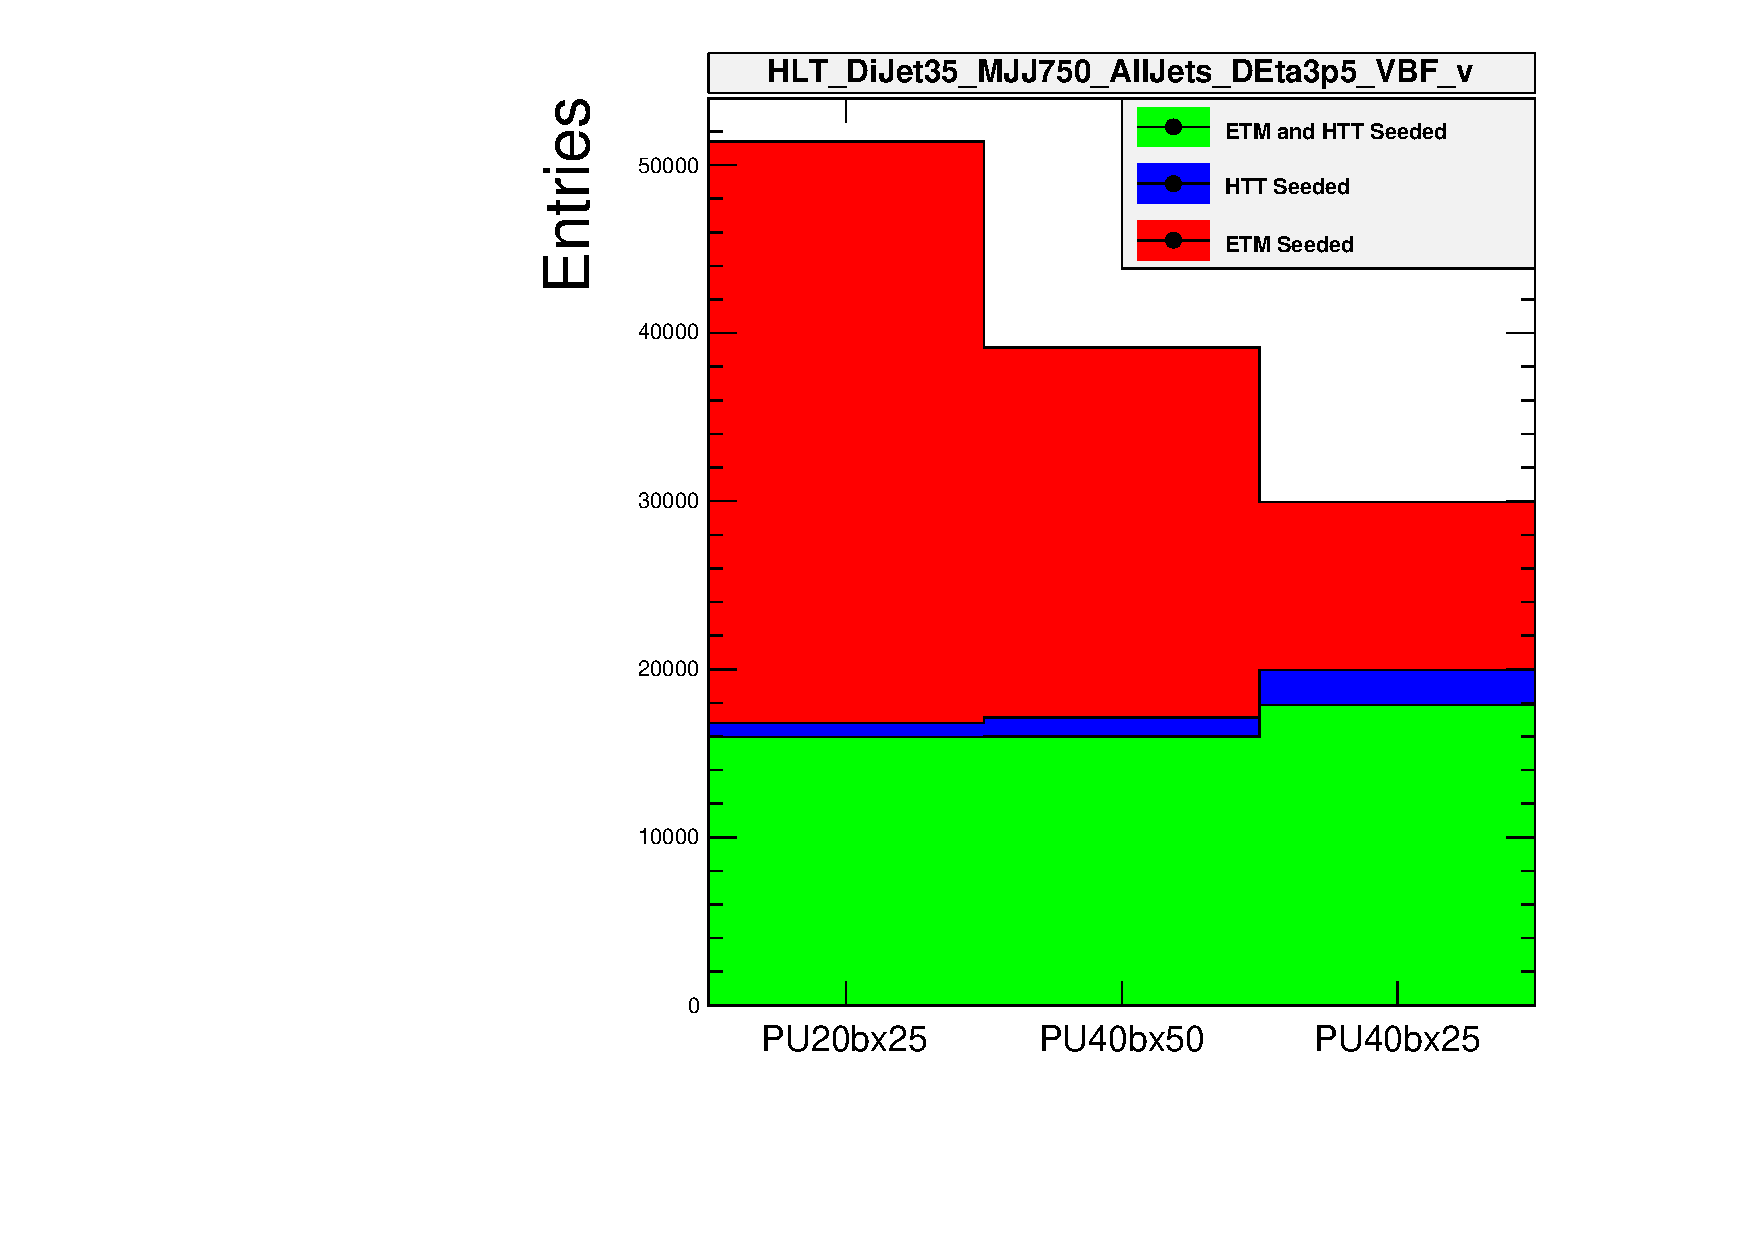
\includegraphics[width=\linewidth]{fig/HLT_DiJet35_MJJ750_AllJets_DEta3p5_VBF_v.pdf}

\end{block}
  
\column[t]{0.45\linewidth}


\end{columns}

\end{frame}

\end{document}